\casesection{Slope effect to bedload transport (2) } 
\label{case:Slopeffect}
\paragraph*{Purpose}
The purpose of this validation case is to examine the performance of D-Flow FM-sed-mor in changing the bedload transport direction due to bed slope  effect in  a straight channel flow simulation; where a symmetric transverse slope has been prescribed through the whole channel length. The test case number is e02-f22-c18.
\paragraph*{Linked claims}
\begin{itemize}
\item The slope effect module gives almost the same result compare to Delft3D software. Due to slope effect, the bedload transport  direction is adjusted towards the direction of the transverse slope, and consequently, the bed level changes. 
\end{itemize} 

\paragraph*{Approach}
Two models have been setup: 
\begin{enumerate}
\item specifying all the input and using D-Flow-sed-mor 4.01.
\item specifying all the input but using D-Flow flexible mesh (FM)-sed-mor module.
\end{enumerate}

\paragraph*{Model description}
A simple structured flexible mesh network for straight channel is built with a length of 16 m and width of 1.6 m. Curvilinear grid also generated similar to FM-net as shown in \Fref{fig:FM_net}. 
\begin{figure}[h!]
\begin{center}
 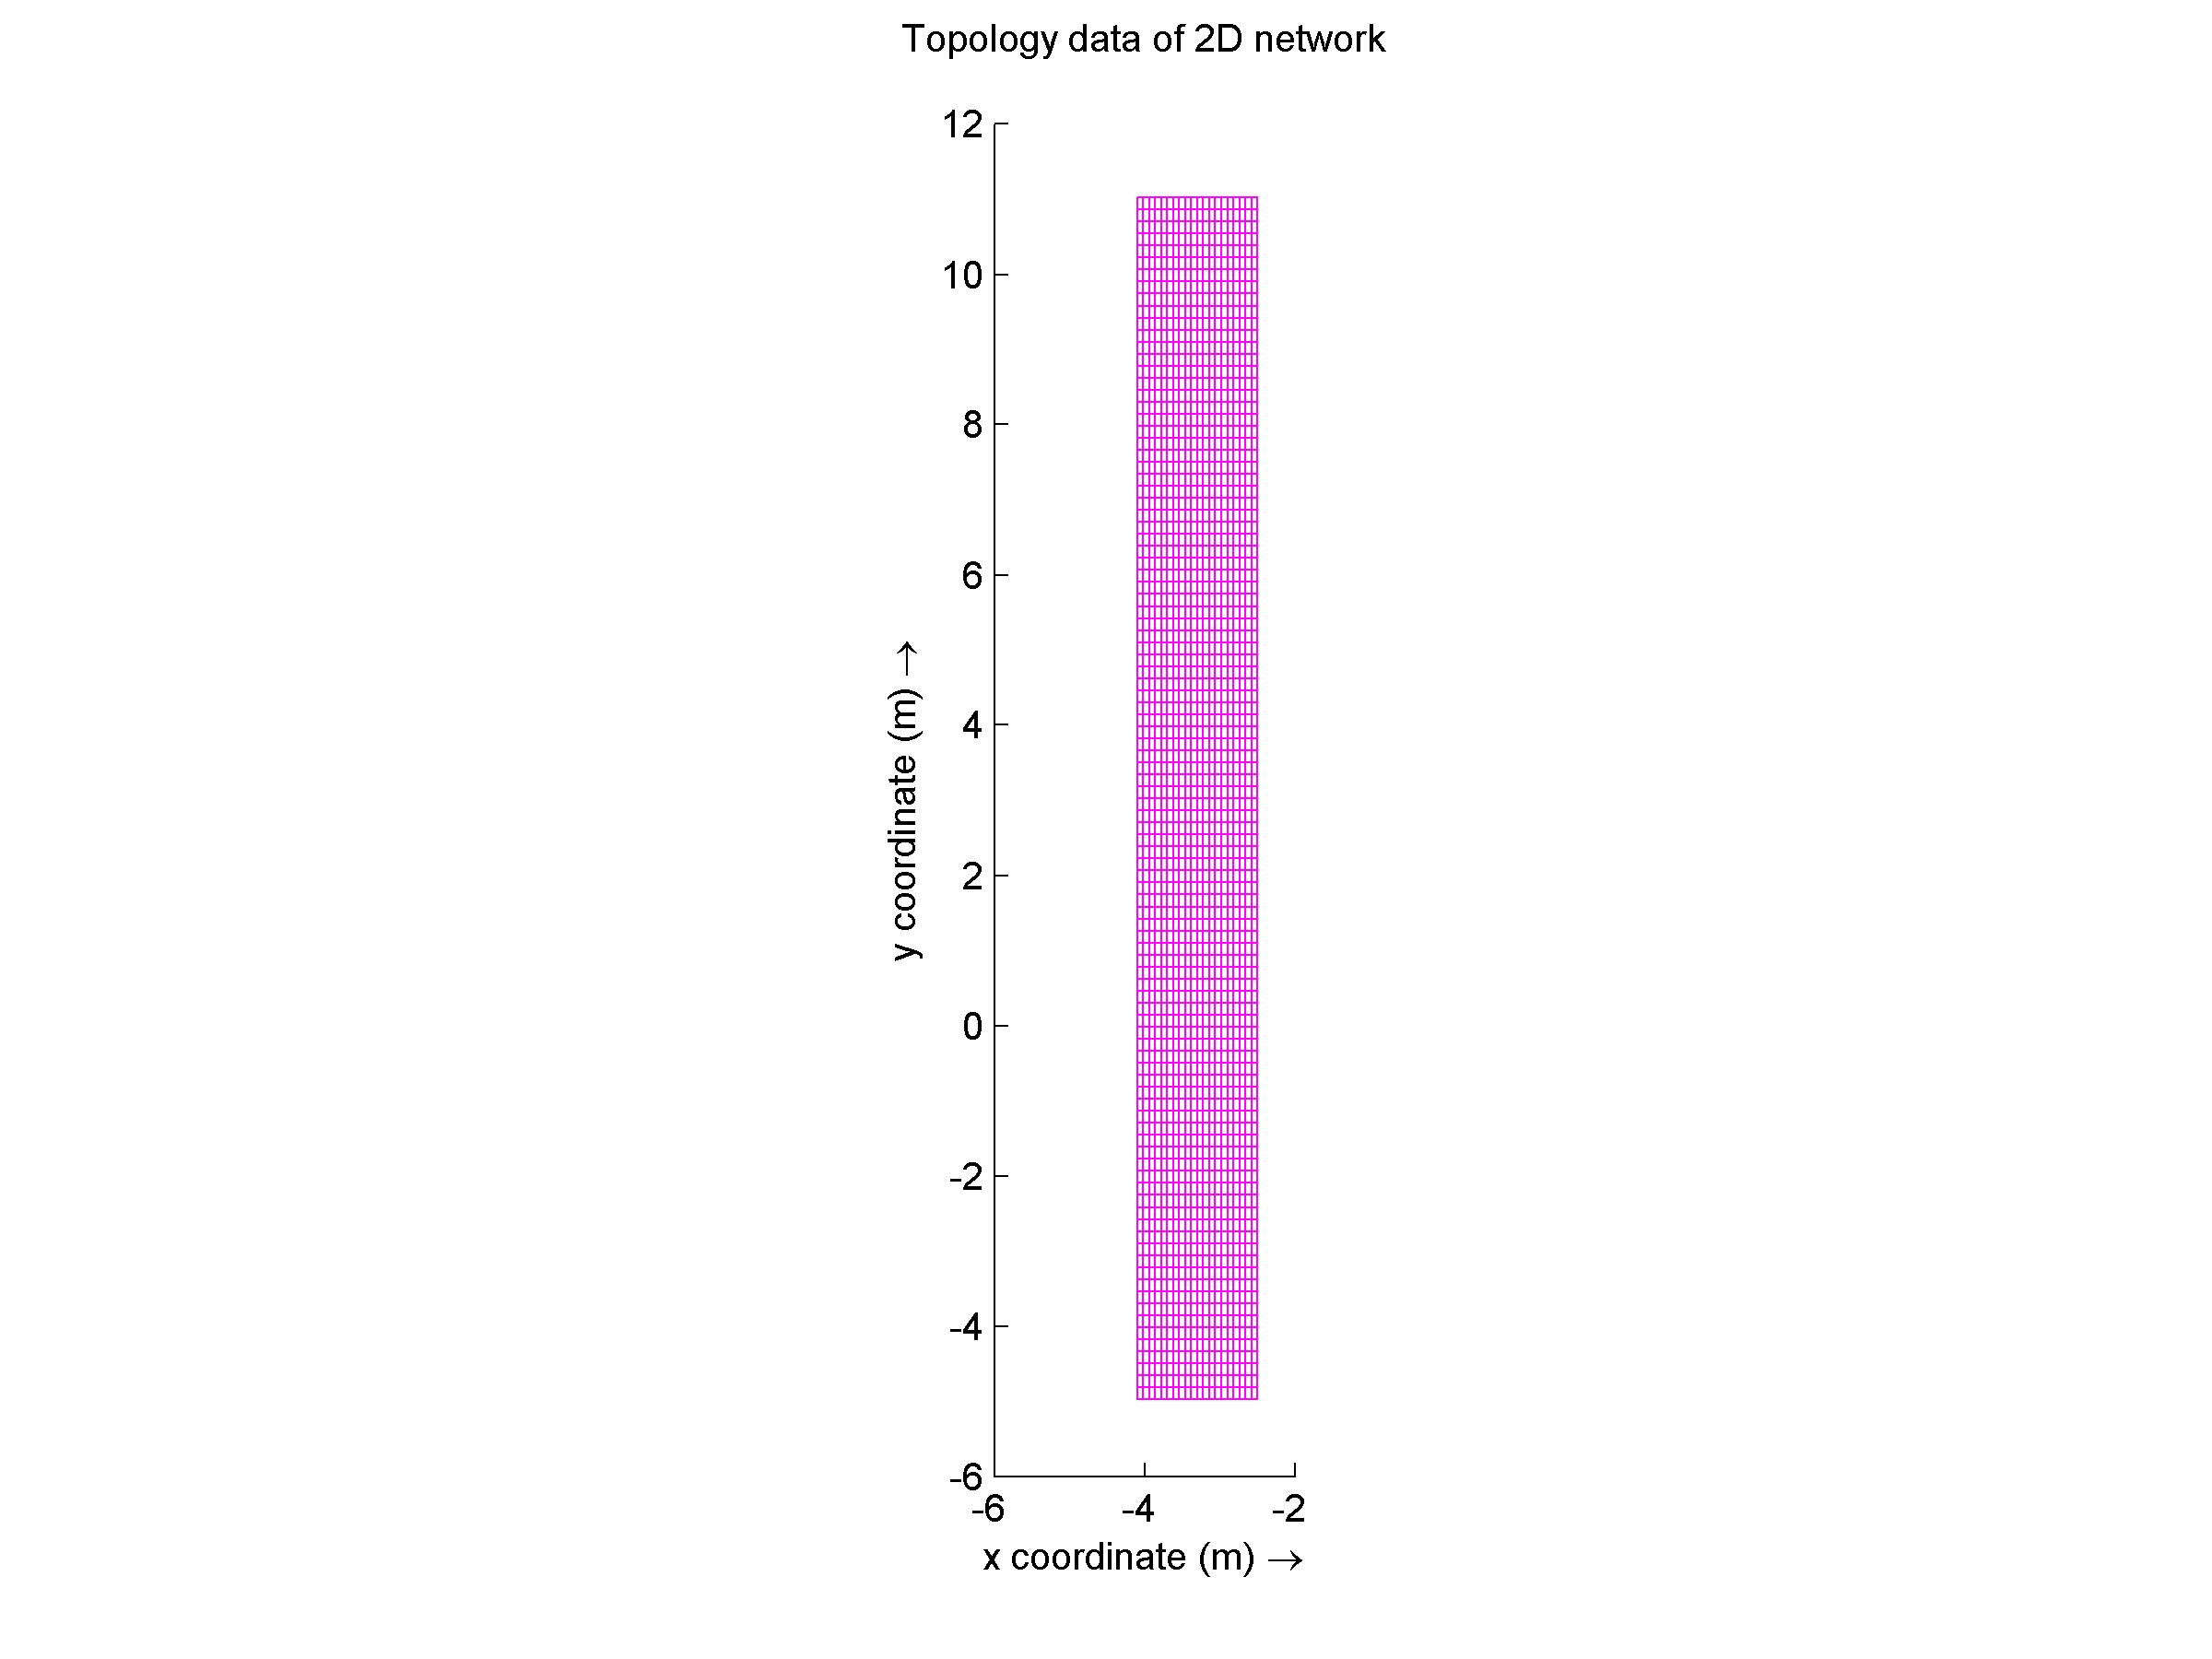
\includegraphics[width=1.0\columnwidth]{fm_net.png}
\end{center}\caption{The network used to test the slope effect.}
\label{fig:FM_net}
\end{figure}
The testcases concern a straight channel flow with a various transverse slopes and a constant roughness factor under equilibrium flow conditions. A discharge $Q$ equal to 2 m$^3$/s is prescribed as upstream boundary condition. The longitudinal bottom slope $i_b$ is prescribed to be $0$. The transverse slope is either 0.22 or 0.44 (see \Fref{fig:initial_bed_level(0.44 and 0.22 transverse slopes)}). The width of the channel is 1.6 m and the corresponding bed level difference at the left and right bank are 0.35 m and 0.7 m for the two respective tranverse slopes. The Ch\'ezy friction coefficient $C$ is set to 60 m$^{1/2}$/s. The downstream boundary condition is water level set to 0.17 m.

\begin{figure}[h!]
\begin{center}
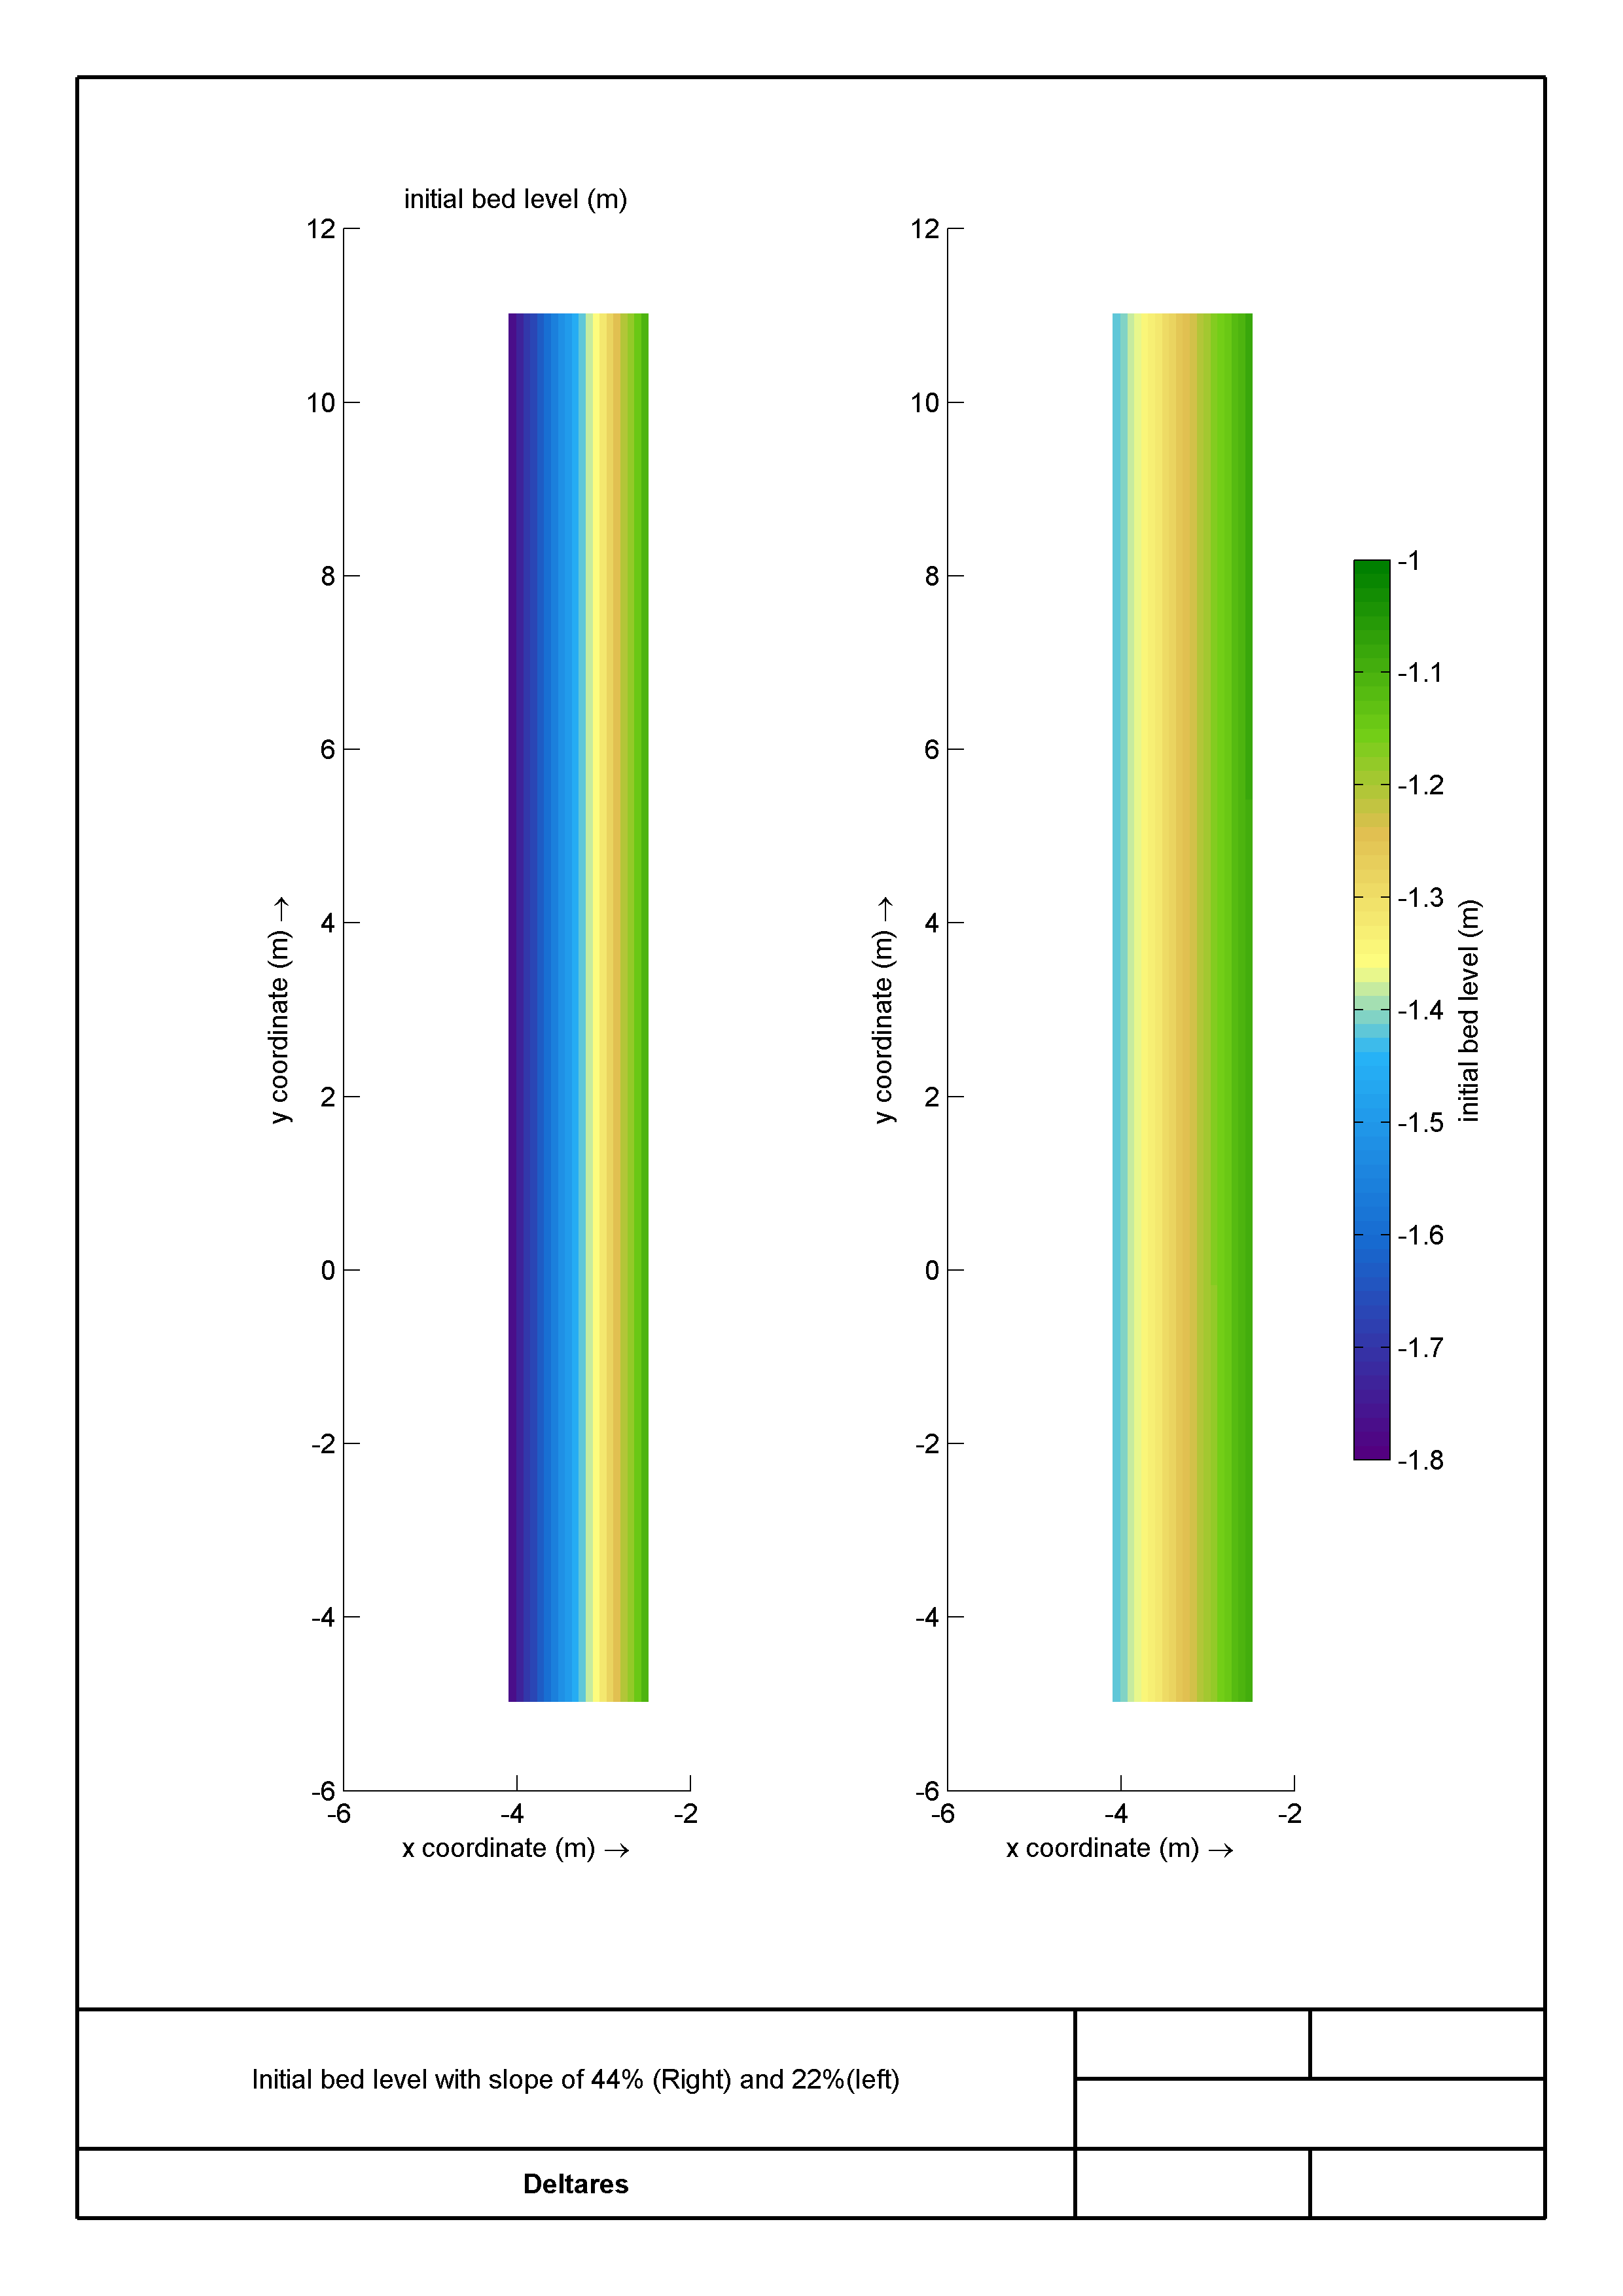
\includegraphics[width=0.7\columnwidth] {initial_bed_level.png}
\end{center}\caption{The initial bed level of the straight channel with transverse slope (TS) of 0.44(on the rightside of the figure) and with (TS) 0.22 (on the right-side of the figure)}
\label{fig:initial_bed_level(0.44 and 0.22 transverse slopes)}
\end{figure}

In addition, an important related setup to morphology file and sediment file used in these testcases are described as follows:
\begin{itemize}
\item[$\bullet$] Sediment file <*.sed>:
\end{itemize}
\begin{verbatim}
[Sediment]
SedTyp           = bedload               # Must be "sand", "mud" or "bedload"
SedDia           = 5.0e-004              # [m] Median sediment diameter (D50)
TraFrm           = 1
Name             = #Engelund-Hansen (1967)#
ACal             = 0.6
RouKs            = 0.08
\end{verbatim}
$SedTyp$ is bedload,
sediment transport equation is Engelund-Hansen (1967),
sediment size ($D_{50}$) is equal to 0.5 mm.
\begin{itemize}
\item[$\bullet$] Morphology file <*.mor>:
\end{itemize}
The morphology update $ MorUpd$ and bed composition update  $CmpUpd$ are off and
$AlfaBs$ is equal to 1 and the bed slope effect is computed by Koch and Flokstra (1980).
\paragraph*{Scenarios without morphological changes}
For testing, five scenarios with different transverse slopes
have been setup,  for the whole bed of the straight channel, and these are described below:
\begin{itemize}
\item[$\bullet$] S0: Transverse flat bed. 
\item[$\bullet$] S1: Transverse slope 0.22 towards right bank.
\item[$\bullet$] S2: Transverse slope 0.44 towards right bank.
\item[$\bullet$] S3: Transverse slope 0.44 in the inverse direction (towards left bank) /(AlfaBs ) is set up to 1. 
\item[$\bullet$] S4: Transverse slope 0.44 in the inverse direction (towards left bank) /(AlfaBs ) is set to 10. 
\end{itemize}
The three different transverse bed slopes have been setup (0, 0.22 and 0.44) alternatively in the scenarios. The slopes 0.22 and 0.44 
are depicted in \Fref{fig:initial_bed_level(0.44 and 0.22 transverse slopes)}. 
The simulation results show that, by comparing the average depth velocity between Delft3D and FM as shown in \Fref{fig:depth_averagedvelocity_d3d(brown)_fm(blue)}, the velocity direction and magnitude are almost similar.

 \begin{figure}[h!]
\begin{center}
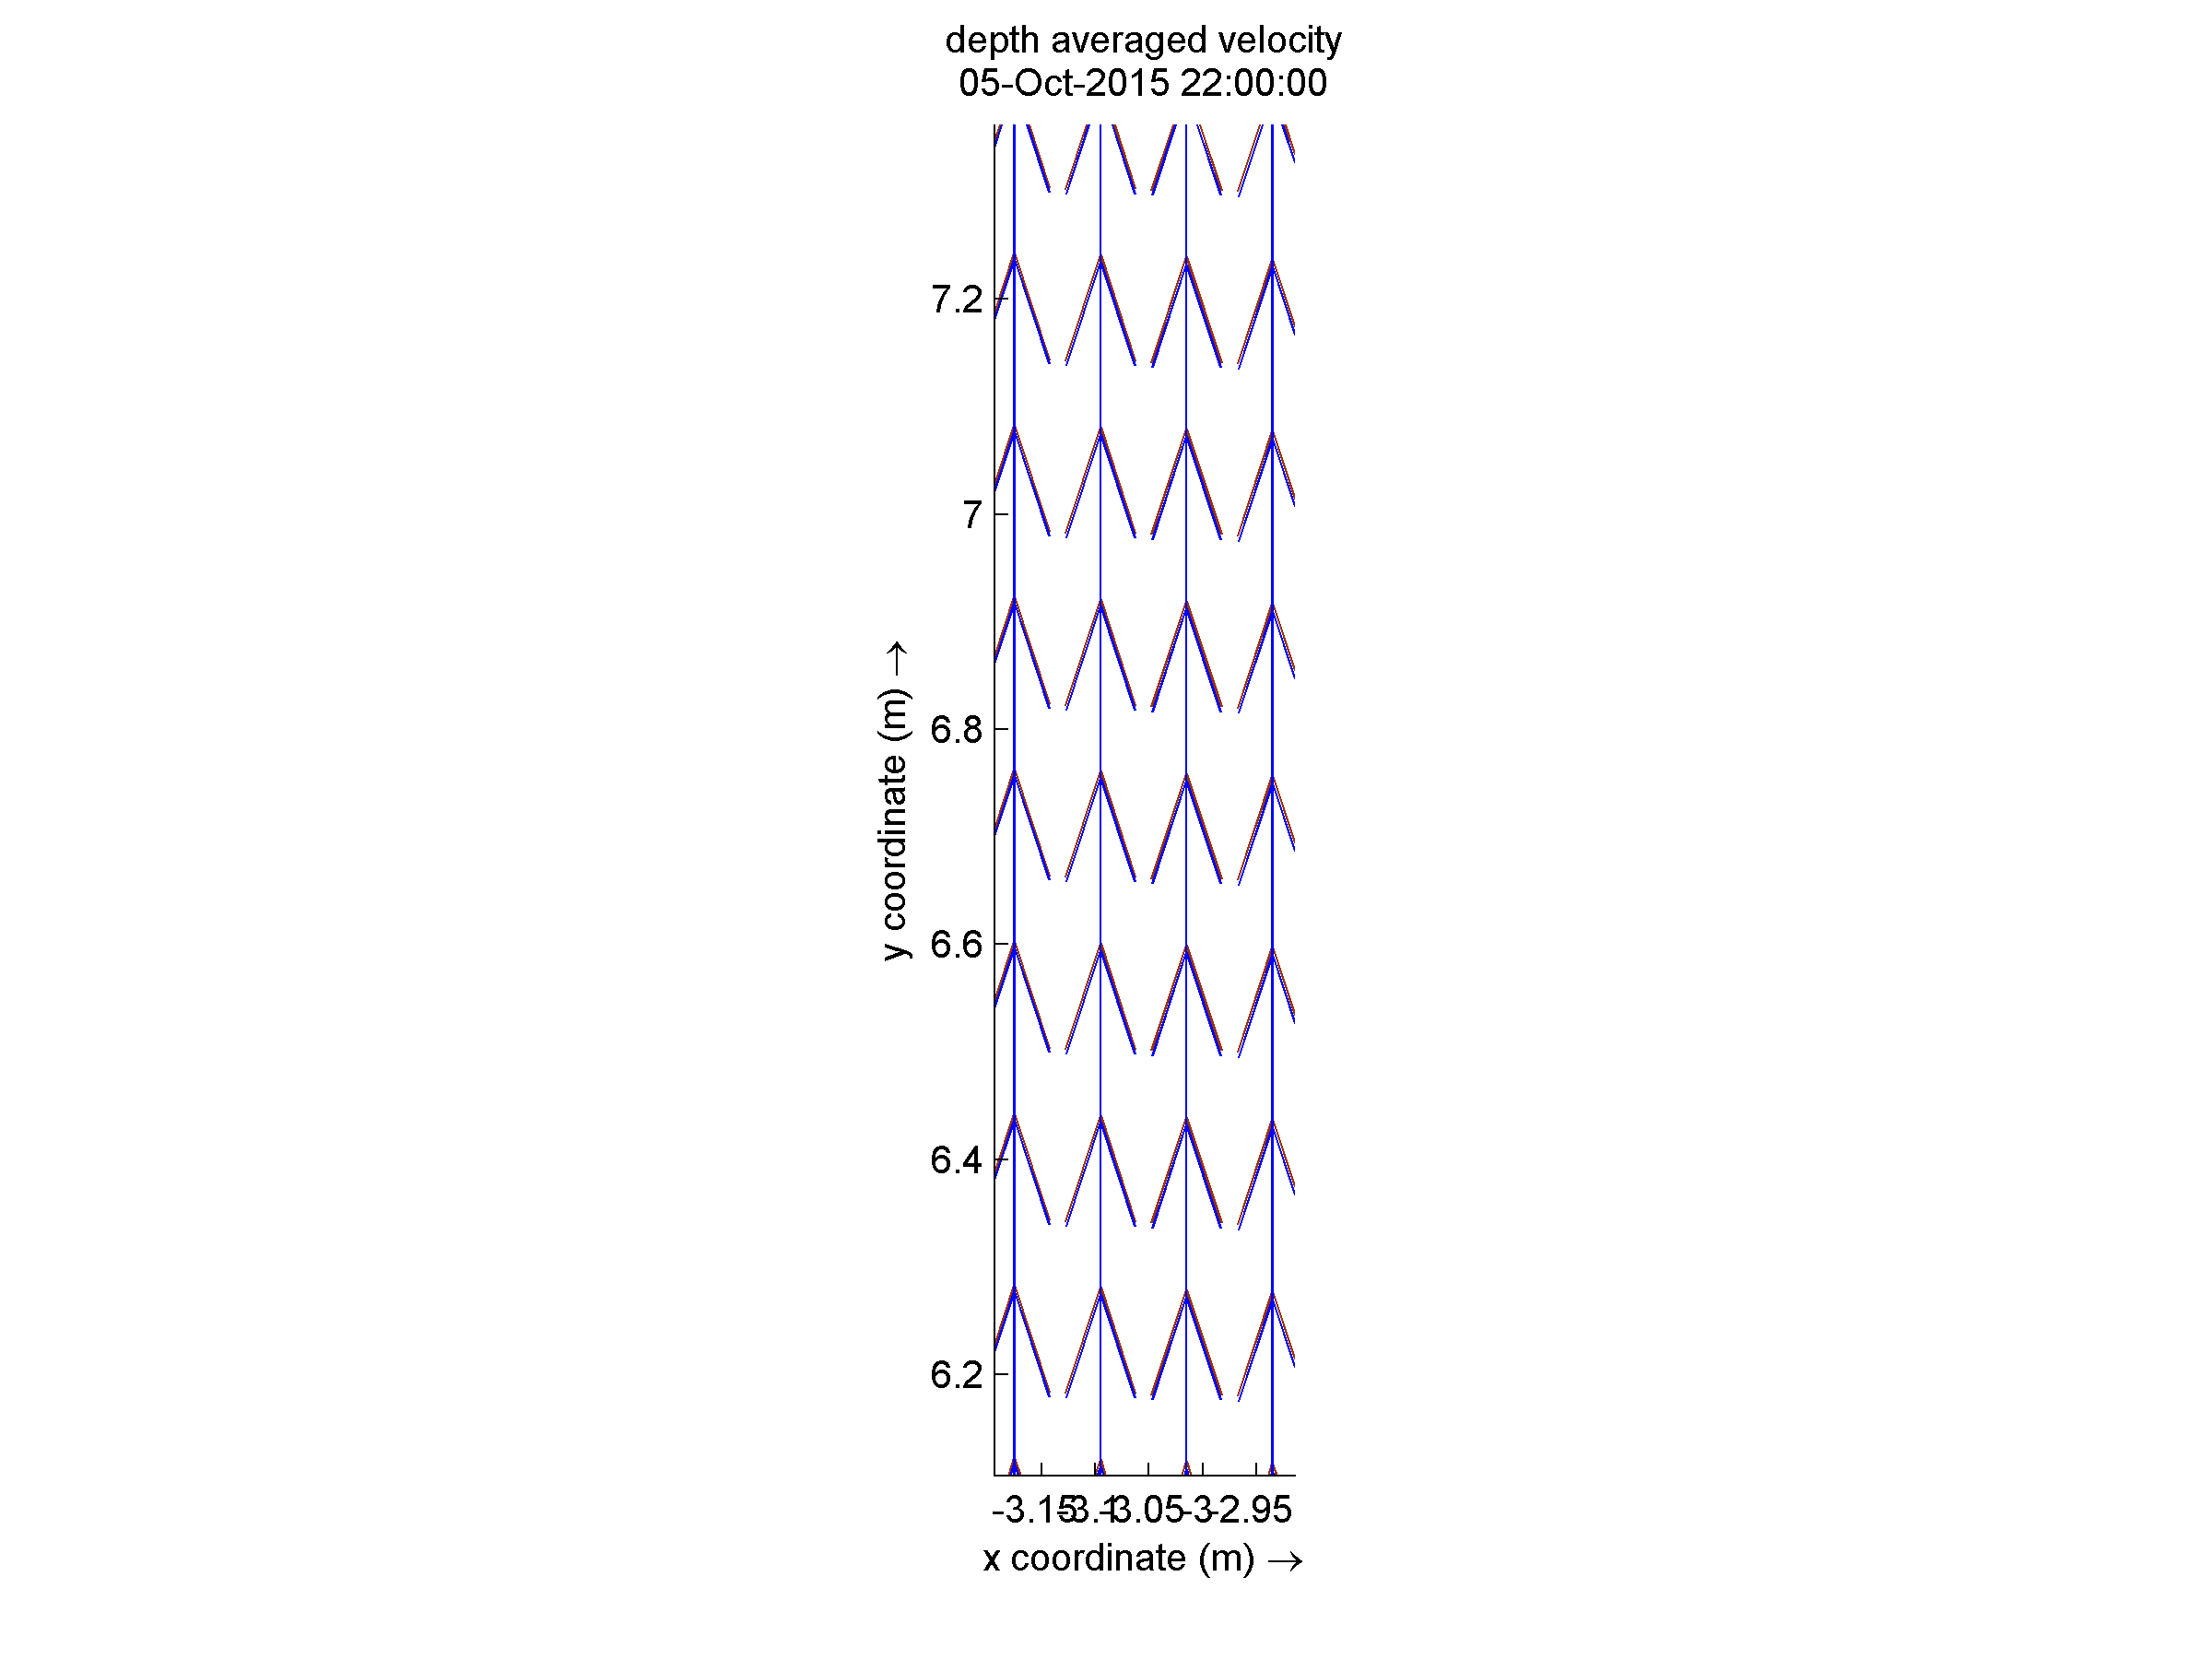
\includegraphics[width=1.0\columnwidth]{depth_averagedvelocity_d3d(brown)_fm(blue).png}
\end{center}\caption{Comparison of depth averaged velocity resulted from two similar simulations of Delft3D (brown line) and FM (blue line)}
\label{fig:depth_averagedvelocity_d3d(brown)_fm(blue)}
\end{figure}

The angle of bedload transport direction is also plotted in \Fref{fig:The bedload transport direction} to display the effect of transverse slope to bedload transport. the  arrows in the figure show the adjustment of bedload transport direction  due to 0, 0.22 and 0.44 transverse slope. The angle of bedload transport twisted towards the expected direction due to transverse slope of the bed .
\Fref{fig:The bedload transport direction with inverseslope} also shows the adjusted direction of the bedload transport when a 0.44 transverse slope is inversed towards the left bank. On the other hand, by comparing the results of Delft3D and FM,the bed load transport direction is same and the arrows are parallel as shown in  \Fref{fig:Bedload_transport_dir_d3dfm22}.
\begin{figure}[h!]
	\begin{center}
    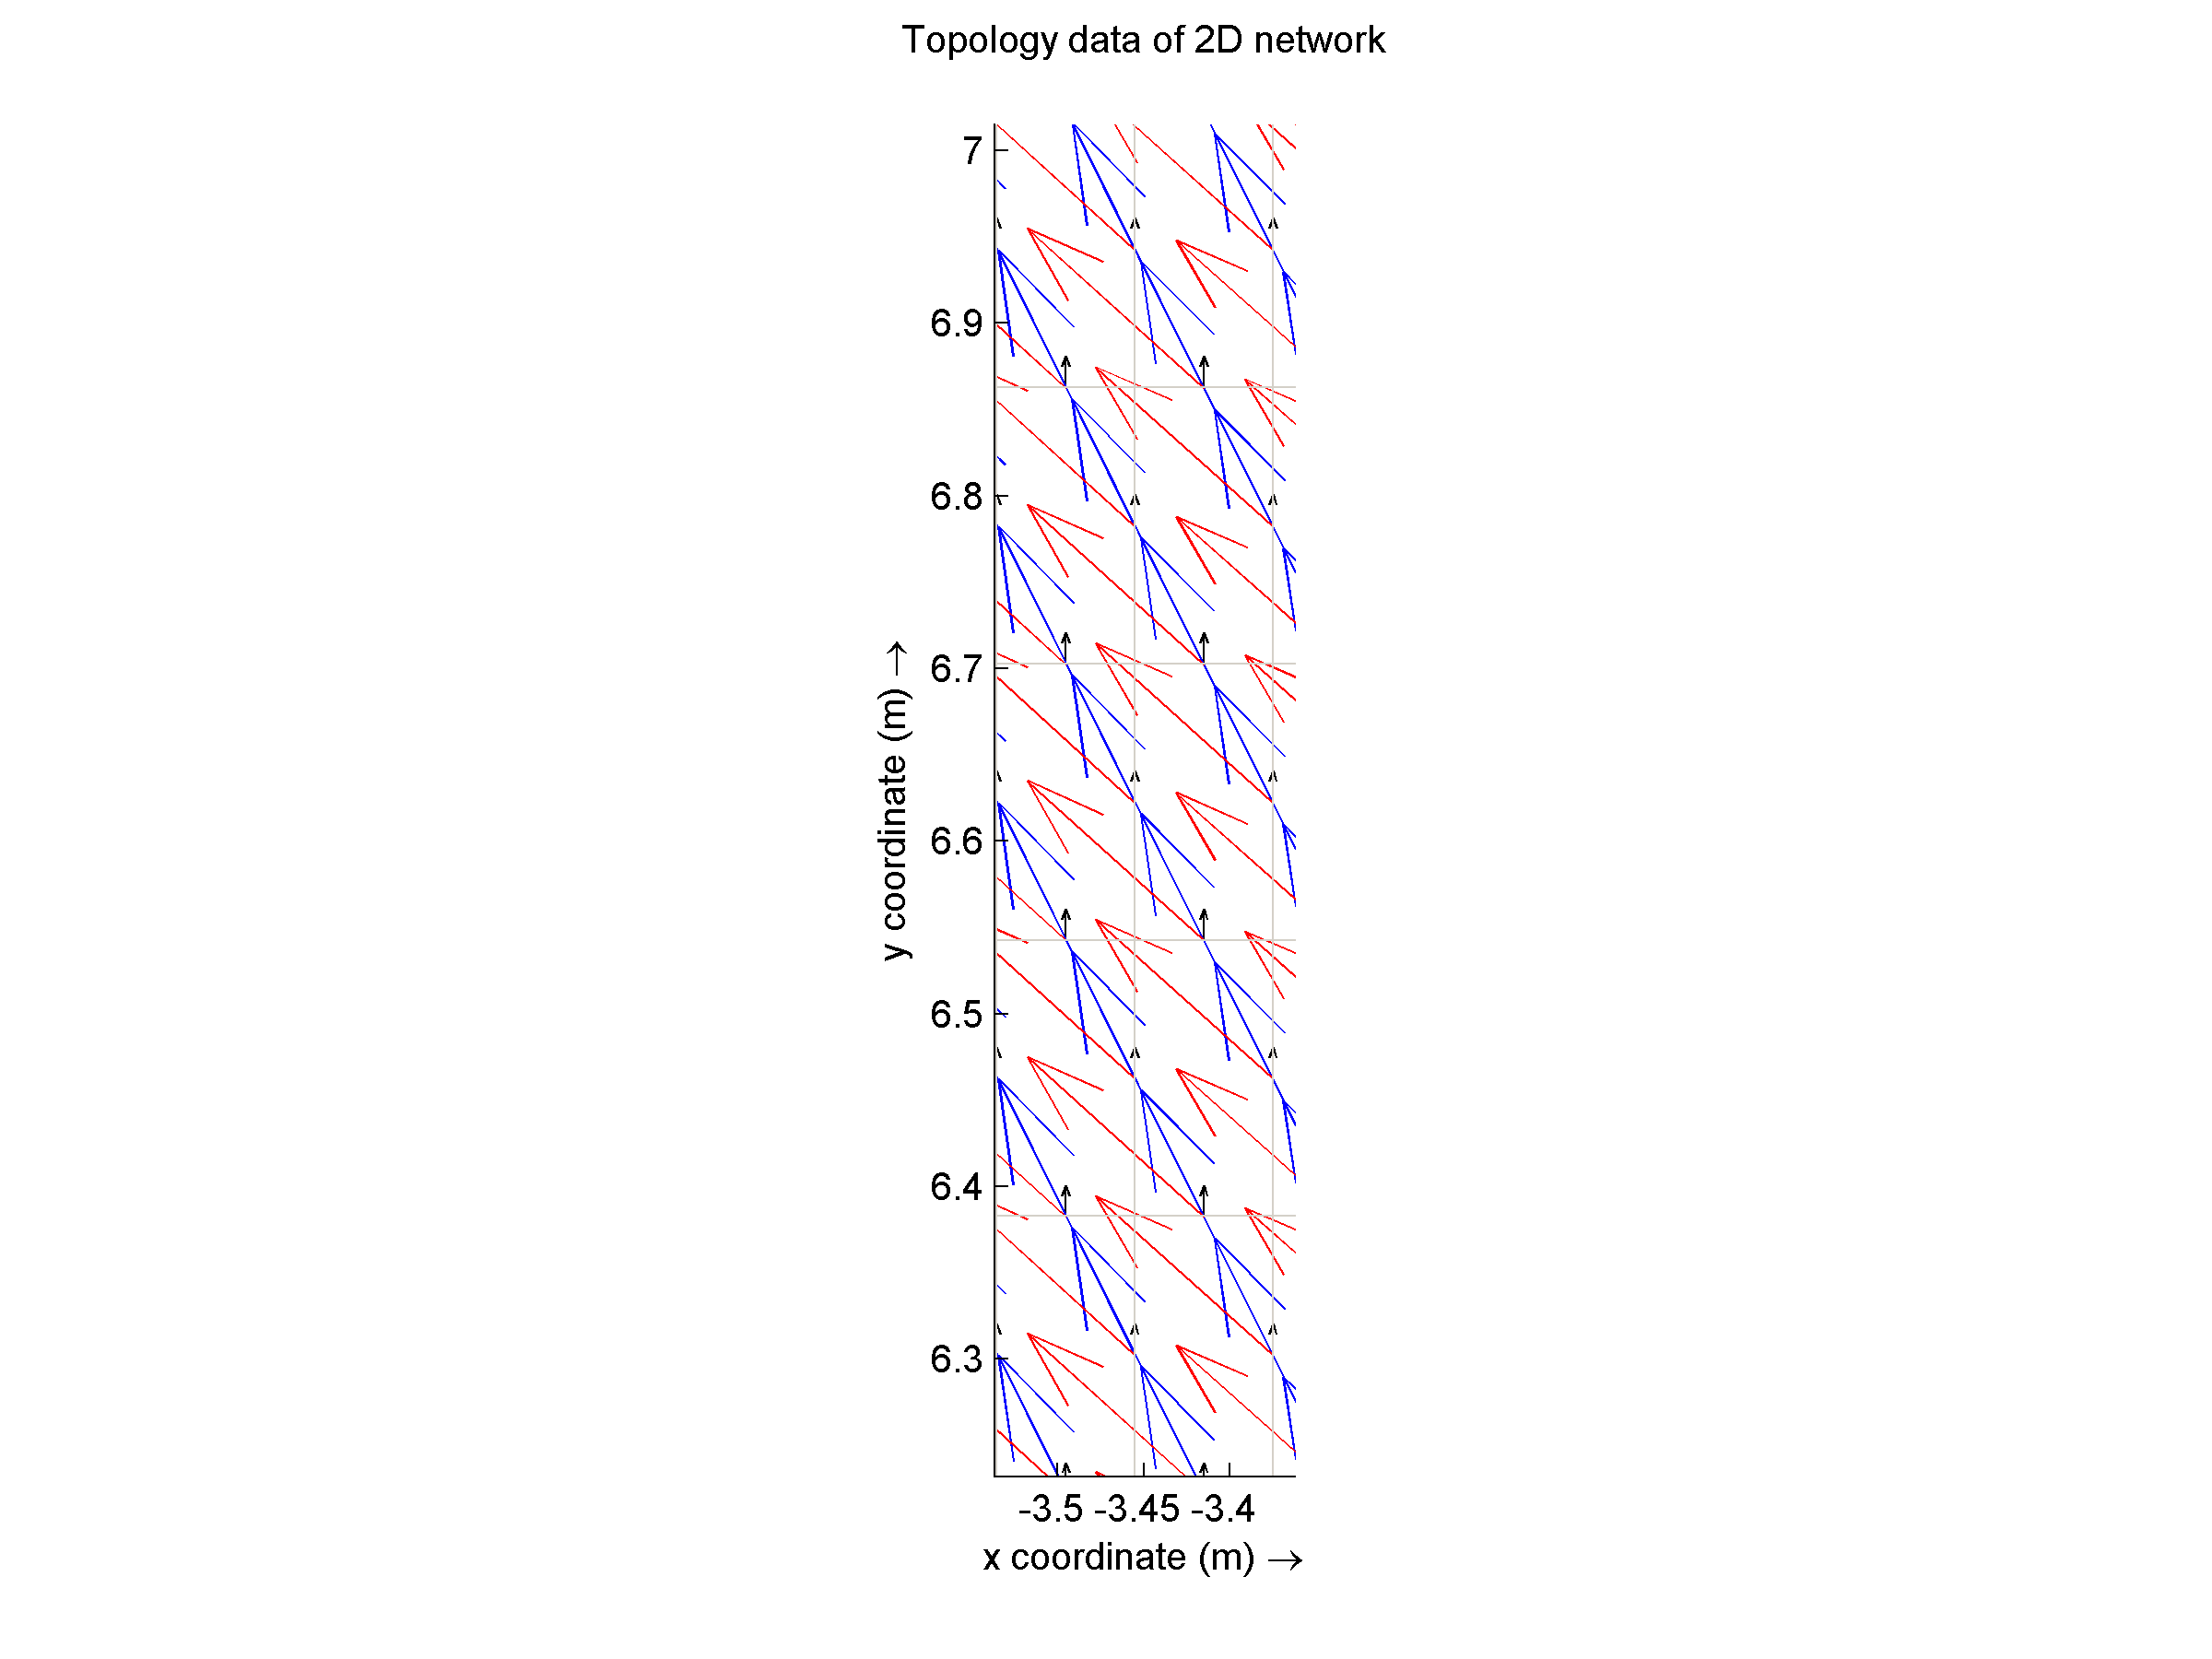
\includegraphics[width=1.0\columnwidth]{bedload_transport_direction.png}
\end{center}\caption{Comparison of bedload transport direction resulted from simulations of FM - 0.22 slope (the blue line), 0.44 slope (the red line) and 0 slope (the black line)}
	\label{fig:The bedload transport direction}
\end{figure}
\begin{figure}[h!]
	\begin{center}
   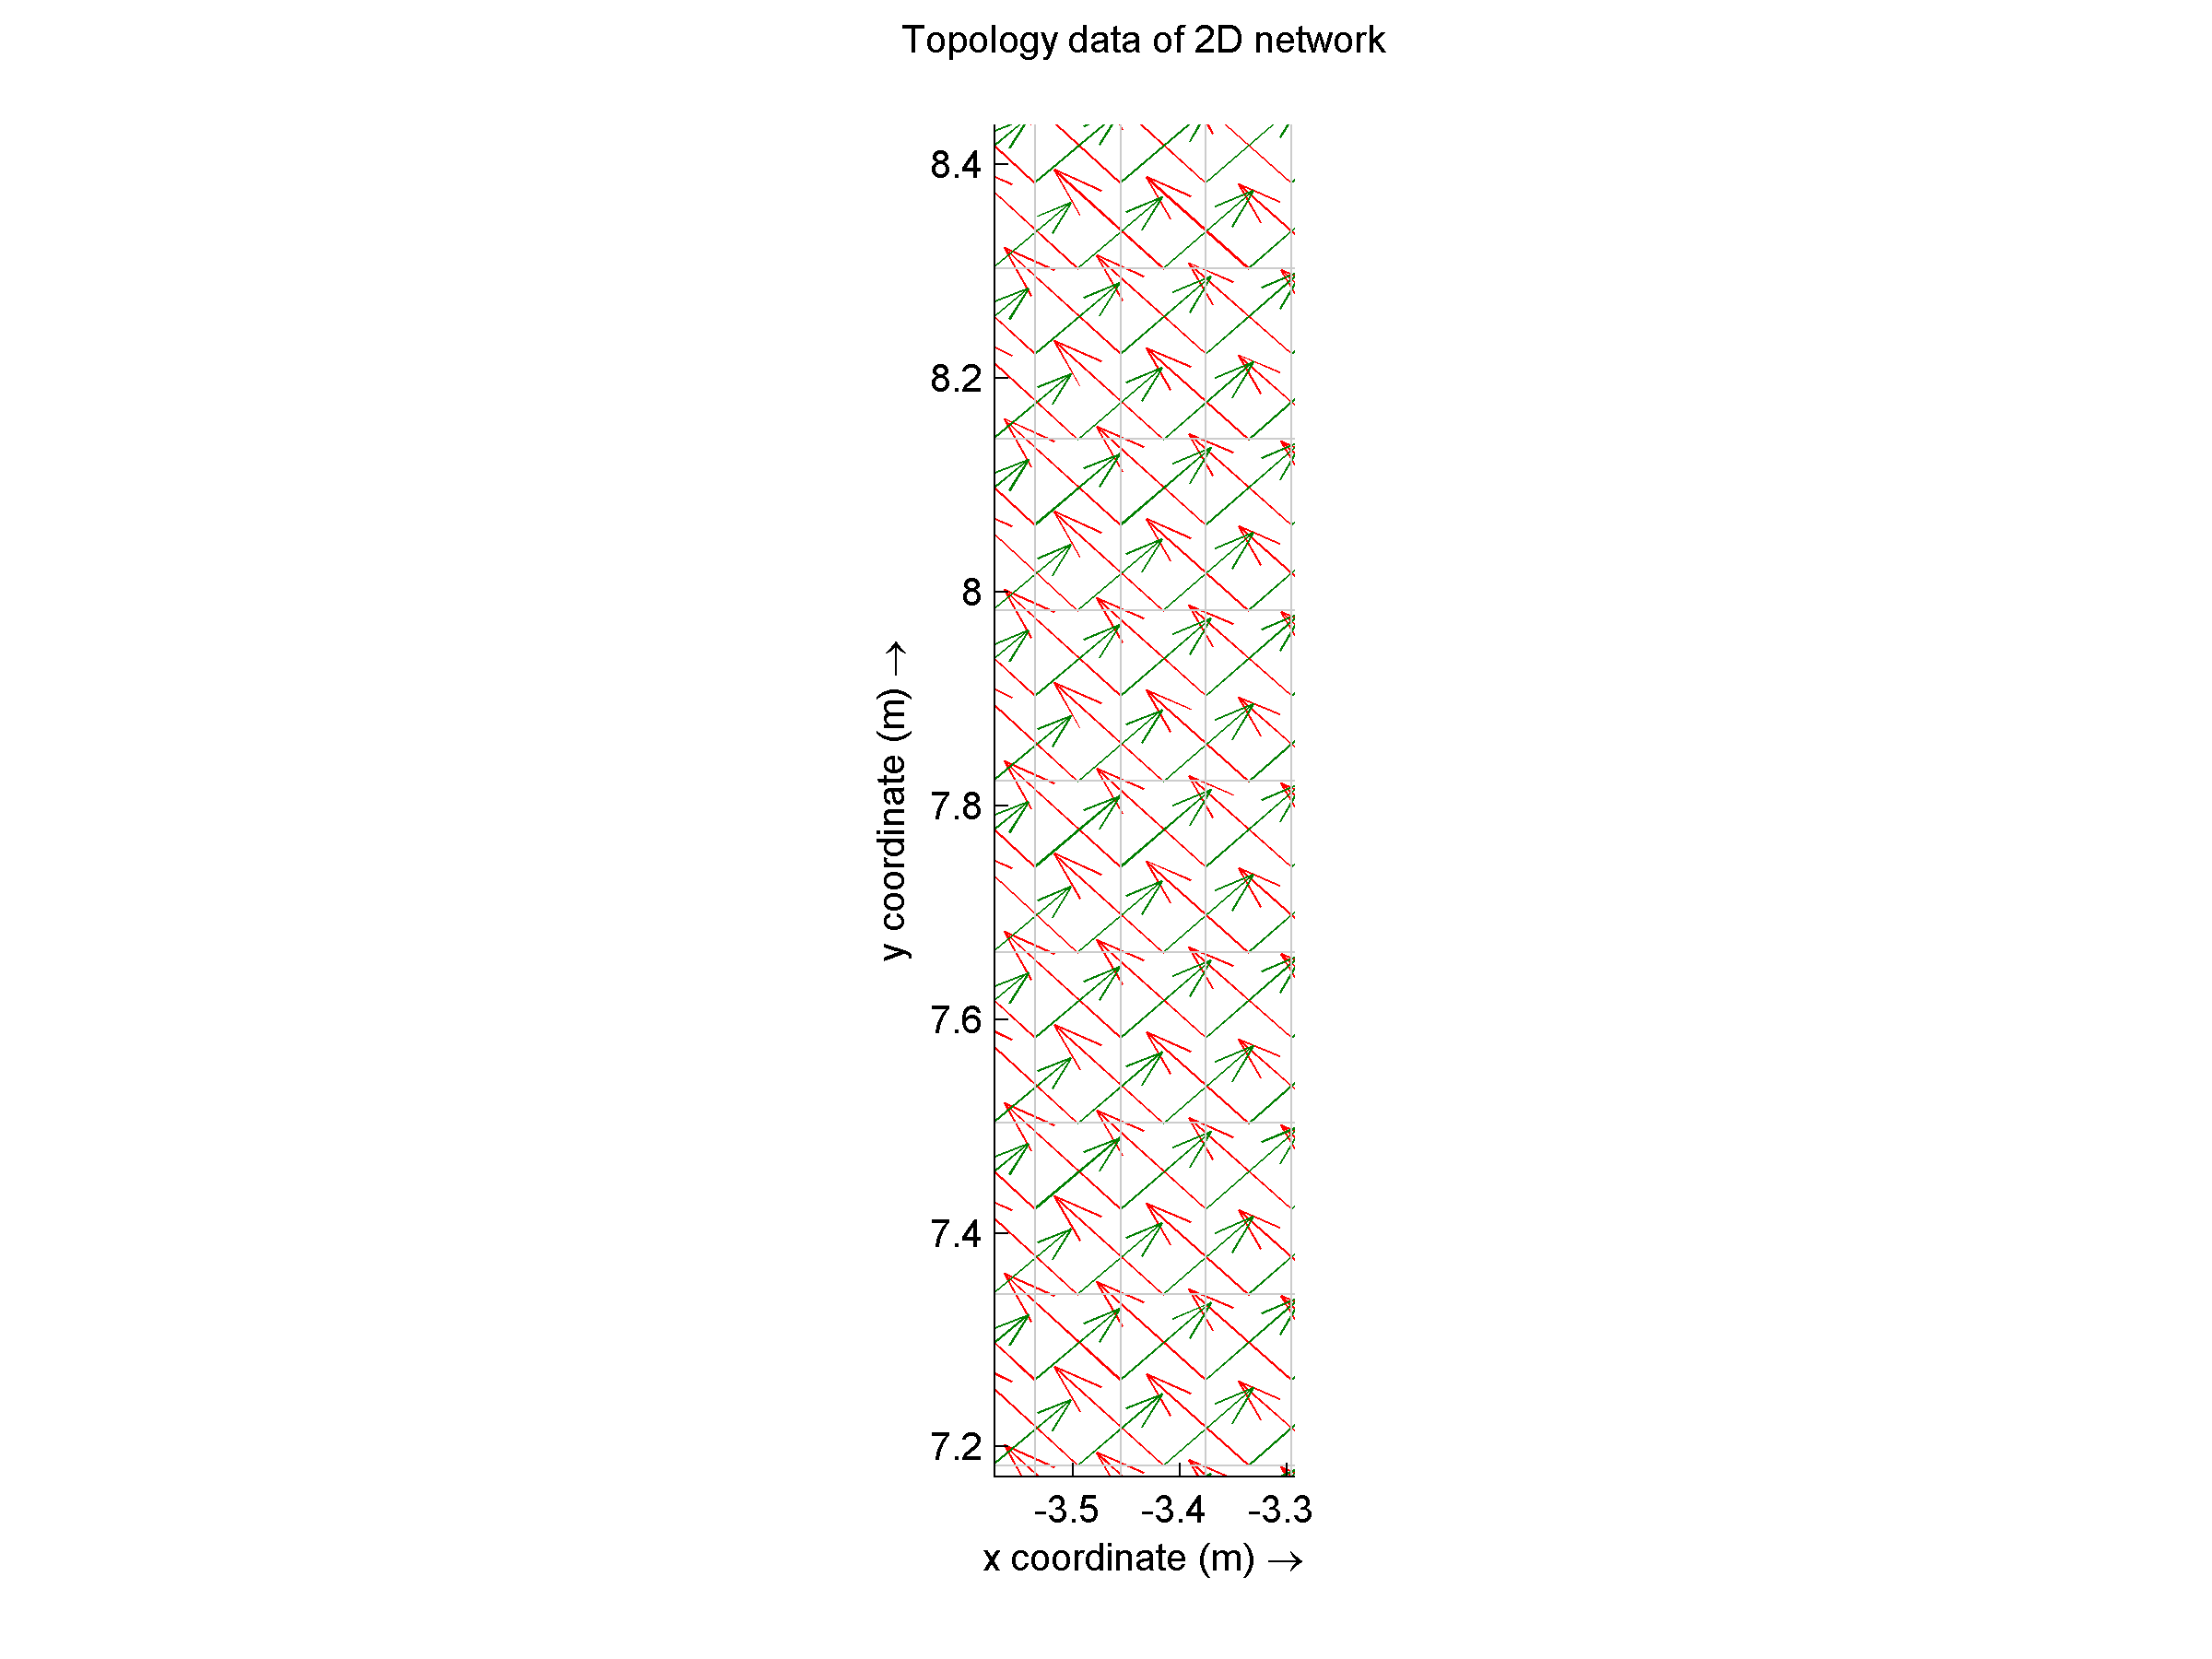
\includegraphics[width=1.0\columnwidth]{bedload_transport_direction_with_inverseslope.png}
	\end{center}\caption{ Comparison of The bedload transport direction with inverse slope resulted from two simulations of FM - 0.4slope towards right bank (the red line) and 0.44slope towards left bank (the green line)}
	\label{fig:The bedload transport direction with inverseslope}
\end{figure}
\begin{figure}[h!]
	\begin{center}
		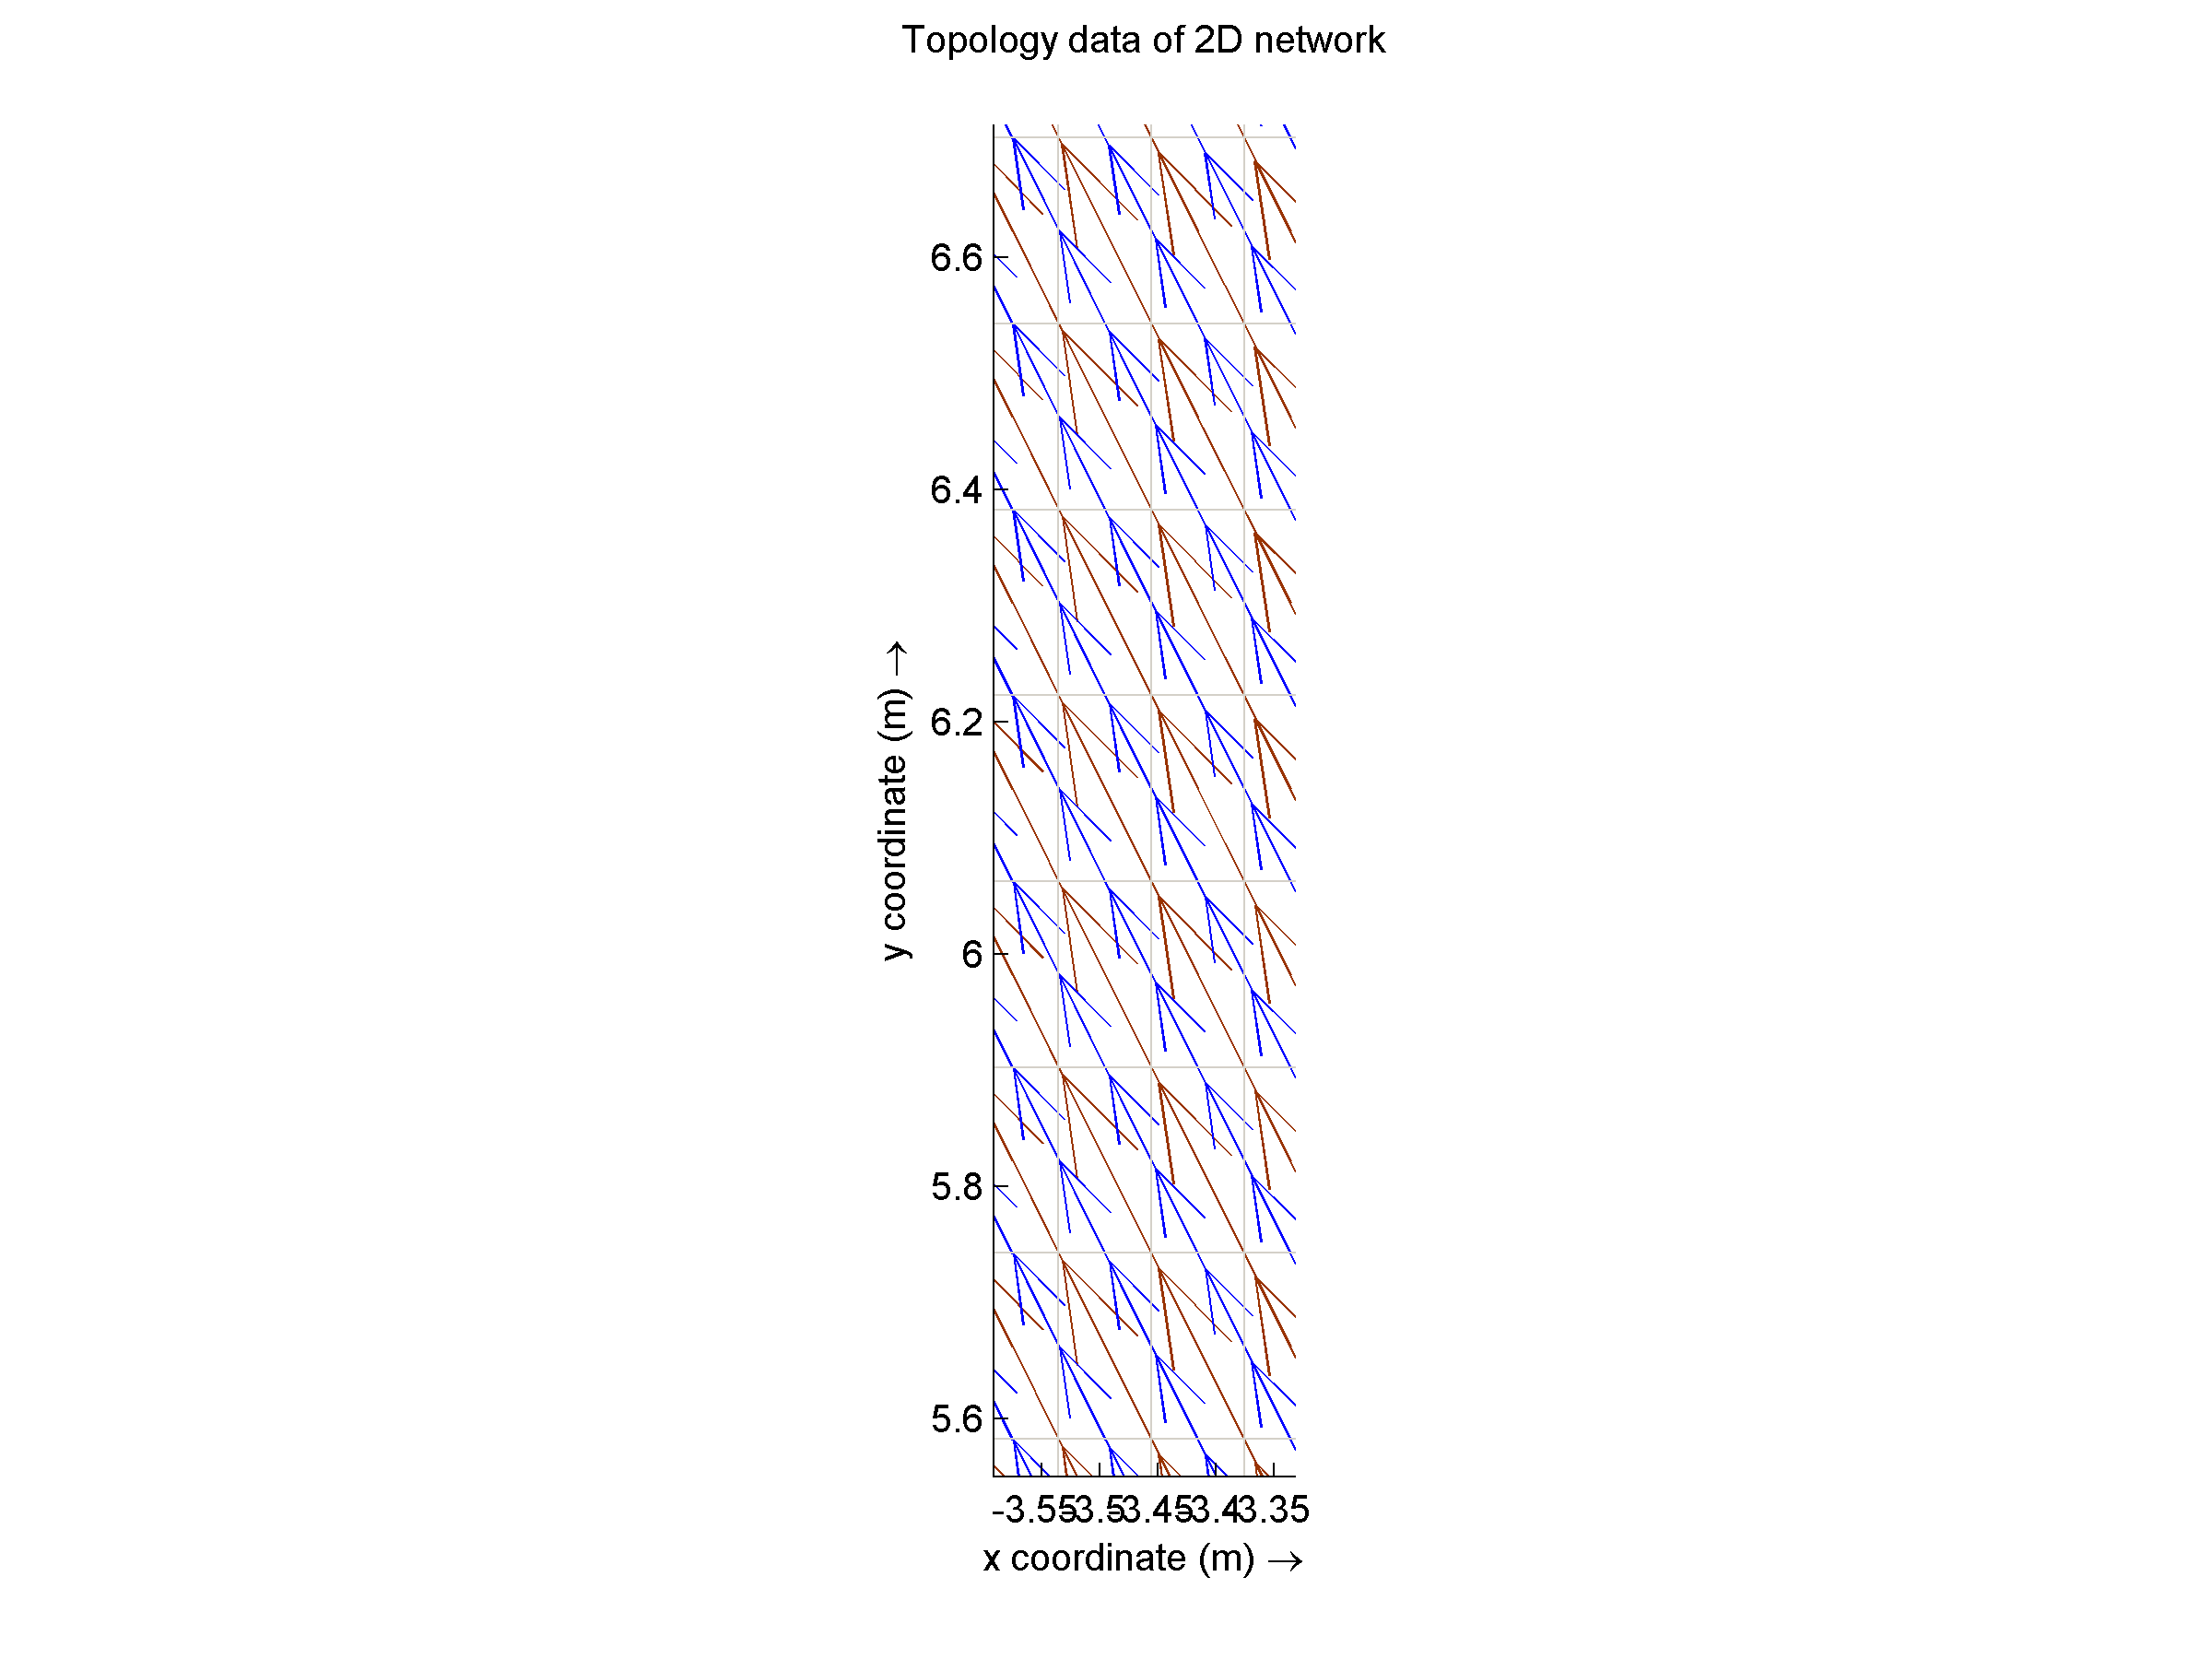
\includegraphics[width=1.0\columnwidth]{Bedload_transport_dir_d3dfm22.png}
	\end{center}\caption{ Comparison of The bedload transport direction  of FM simulation(the blue line) and Delft3D simulation (the brown line)}
	\label{fig:Bedload_transport_dir_d3dfm22}
\end{figure}
\begin{figure}[h!]
 \begin{center}	 
   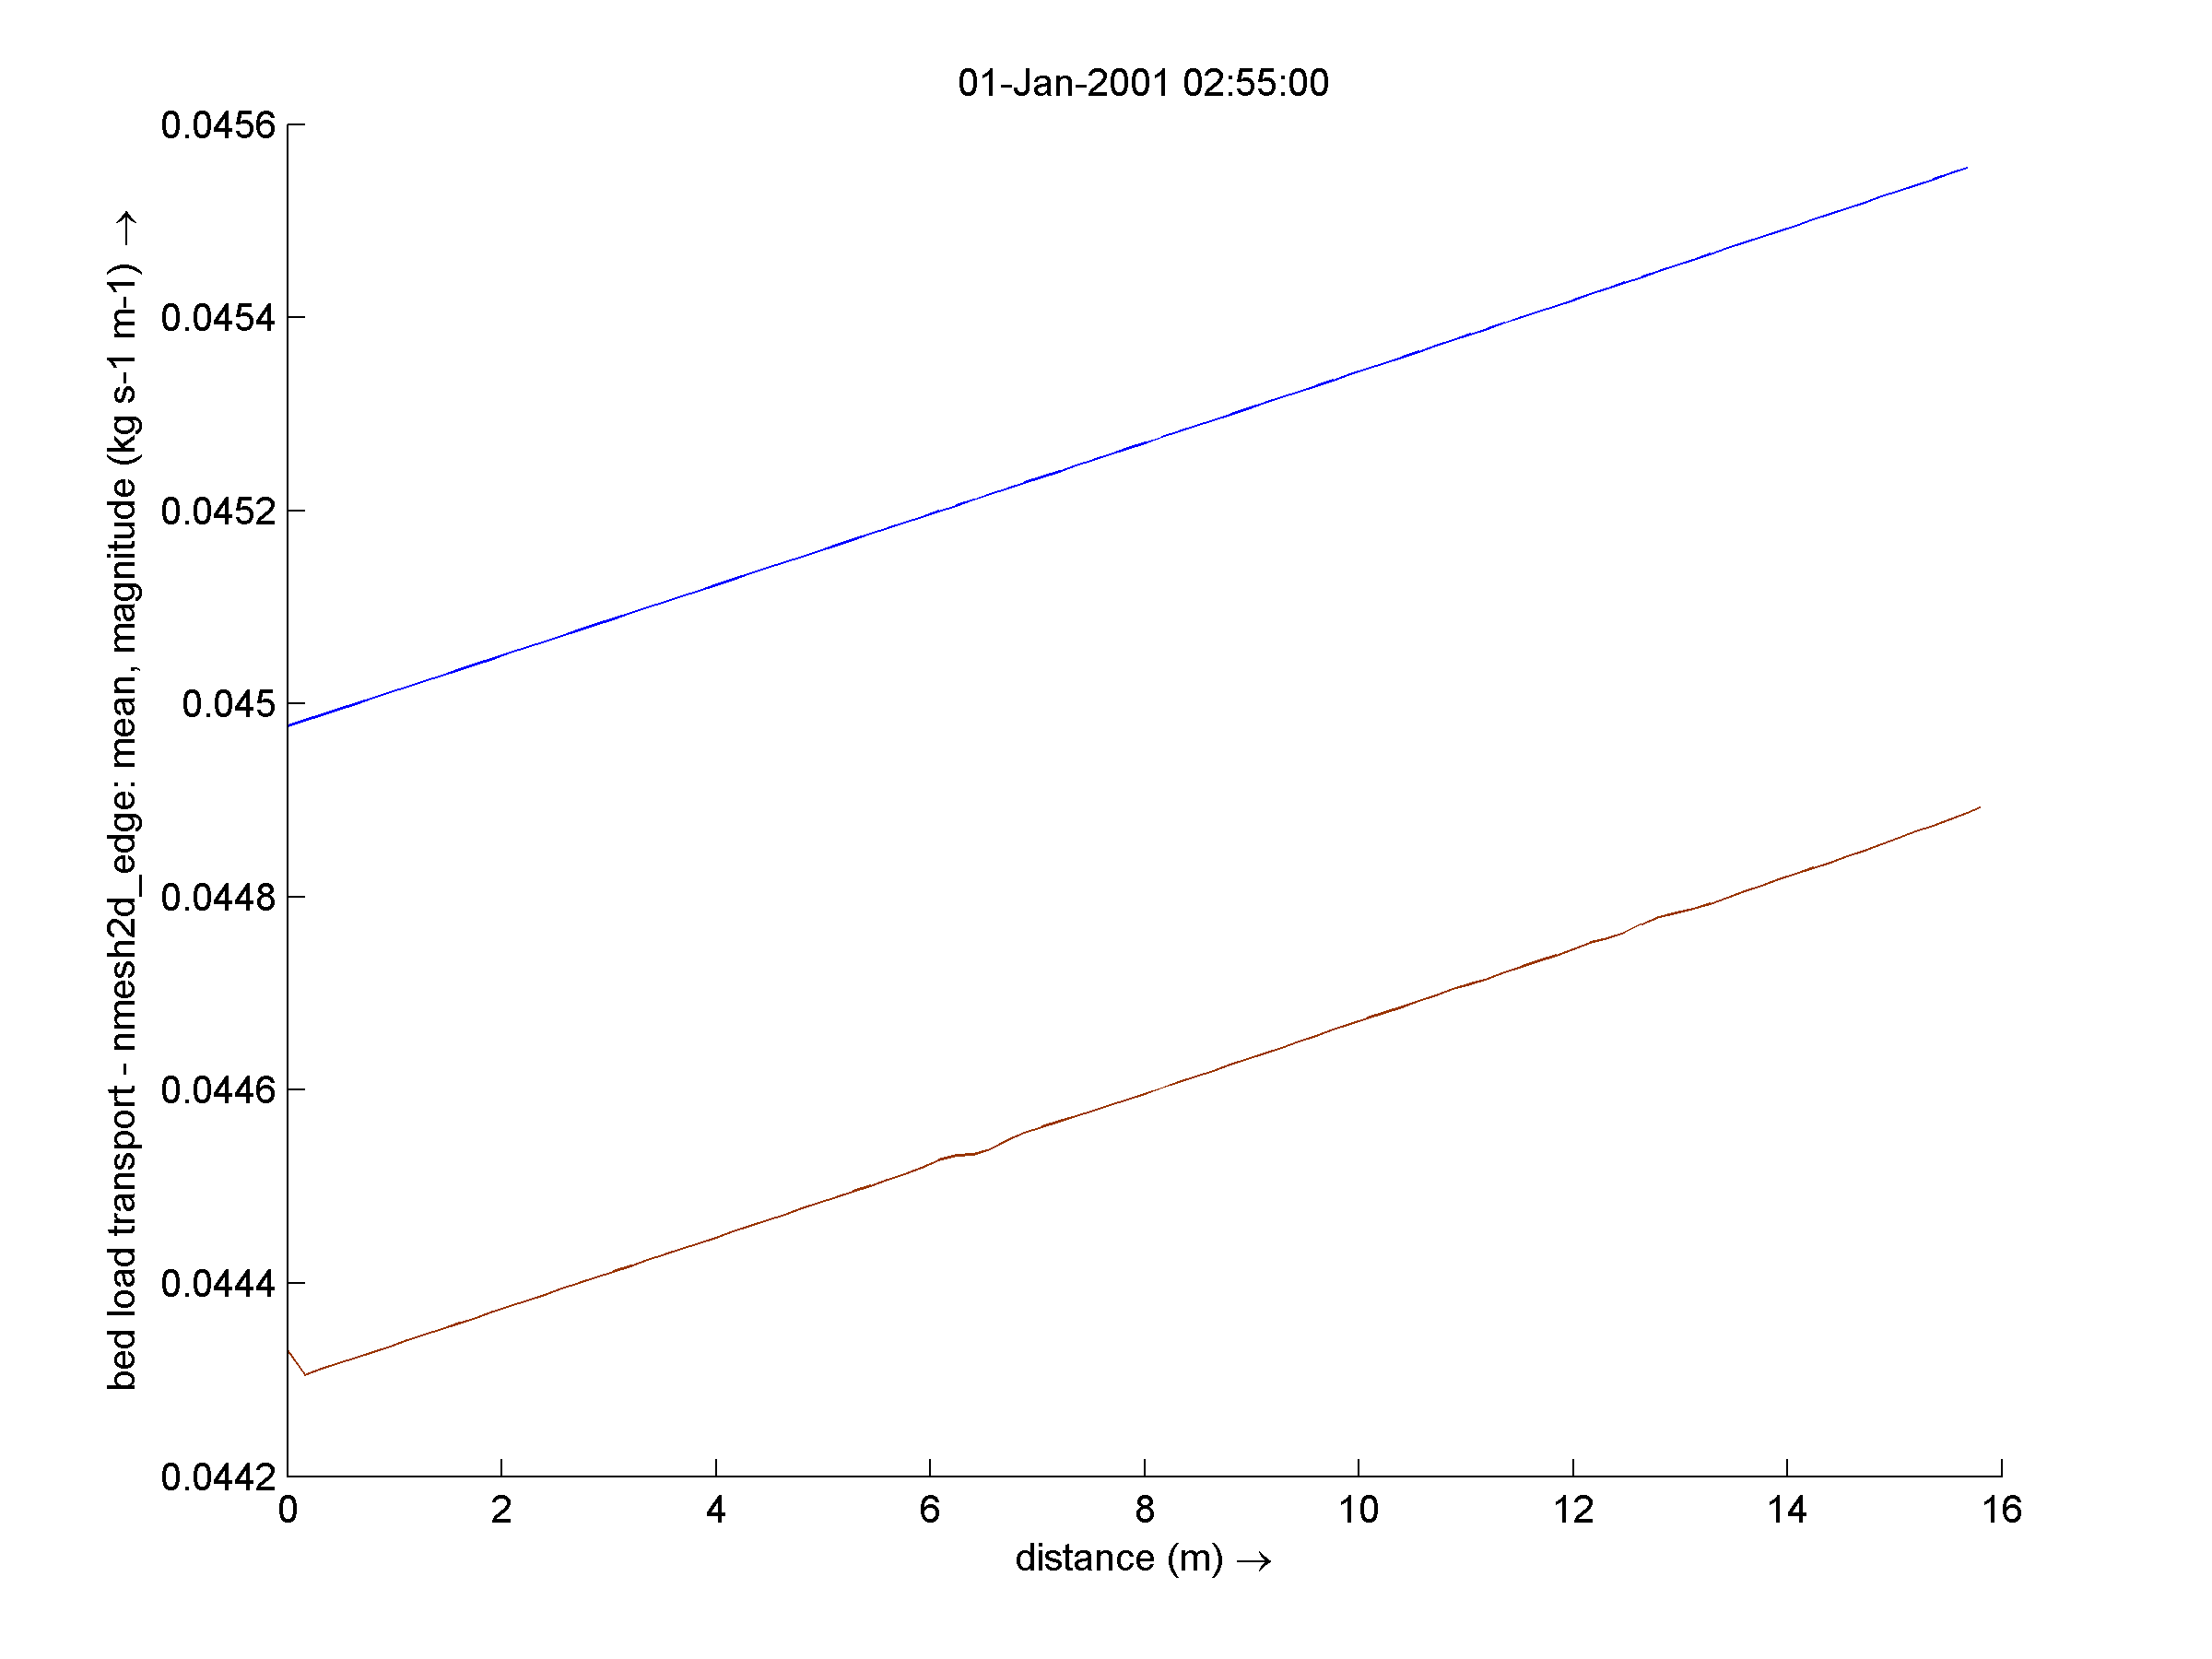
\includegraphics[width=0.7\columnwidth]{bedloadtransport-magnitude-centreline-strchannel.png}
\end{center}\caption {Comparison of The bedload transport magnitude in the centreline of the straight channel (brown line) and FM (blue line)}
		\label{fig:bedloadtransport-magnitude-centreline-strchannel}
  \end{figure} 
\par The magnitude of bedload transport in the D-Flow FM is deviated by 1.5 $\%$ from the Delft3D software.This is illustrated in
\Fref{fig:bedloadtransport-magnitude-centreline-strchannel}, where the magnitude is plotted by selecting the stream centreline of the straight channel with
transverse slope of 22$\%$.\par Furthermore, Delft3D and FM bedload transport were checked against Engelund-Hansen (1967) bedload transport equation as shown in \Fref{fig:velocity_bedloadtransport_plot}. The depth average velocity and bedload transport, at the streamline of the channel, were exported from Delft3D and FM models, and then compared with calculated bedload transport corresponding to various velocities using Engelund-Hansen formula. The result shows that the FM model with a certain velocity gives a good result of bedload transport, while Delft3D bedload transport is less than what is calculated using Engelund-Hansen (1967) formula.
    \begin{figure}[h!]
    	\begin{center}	 
    		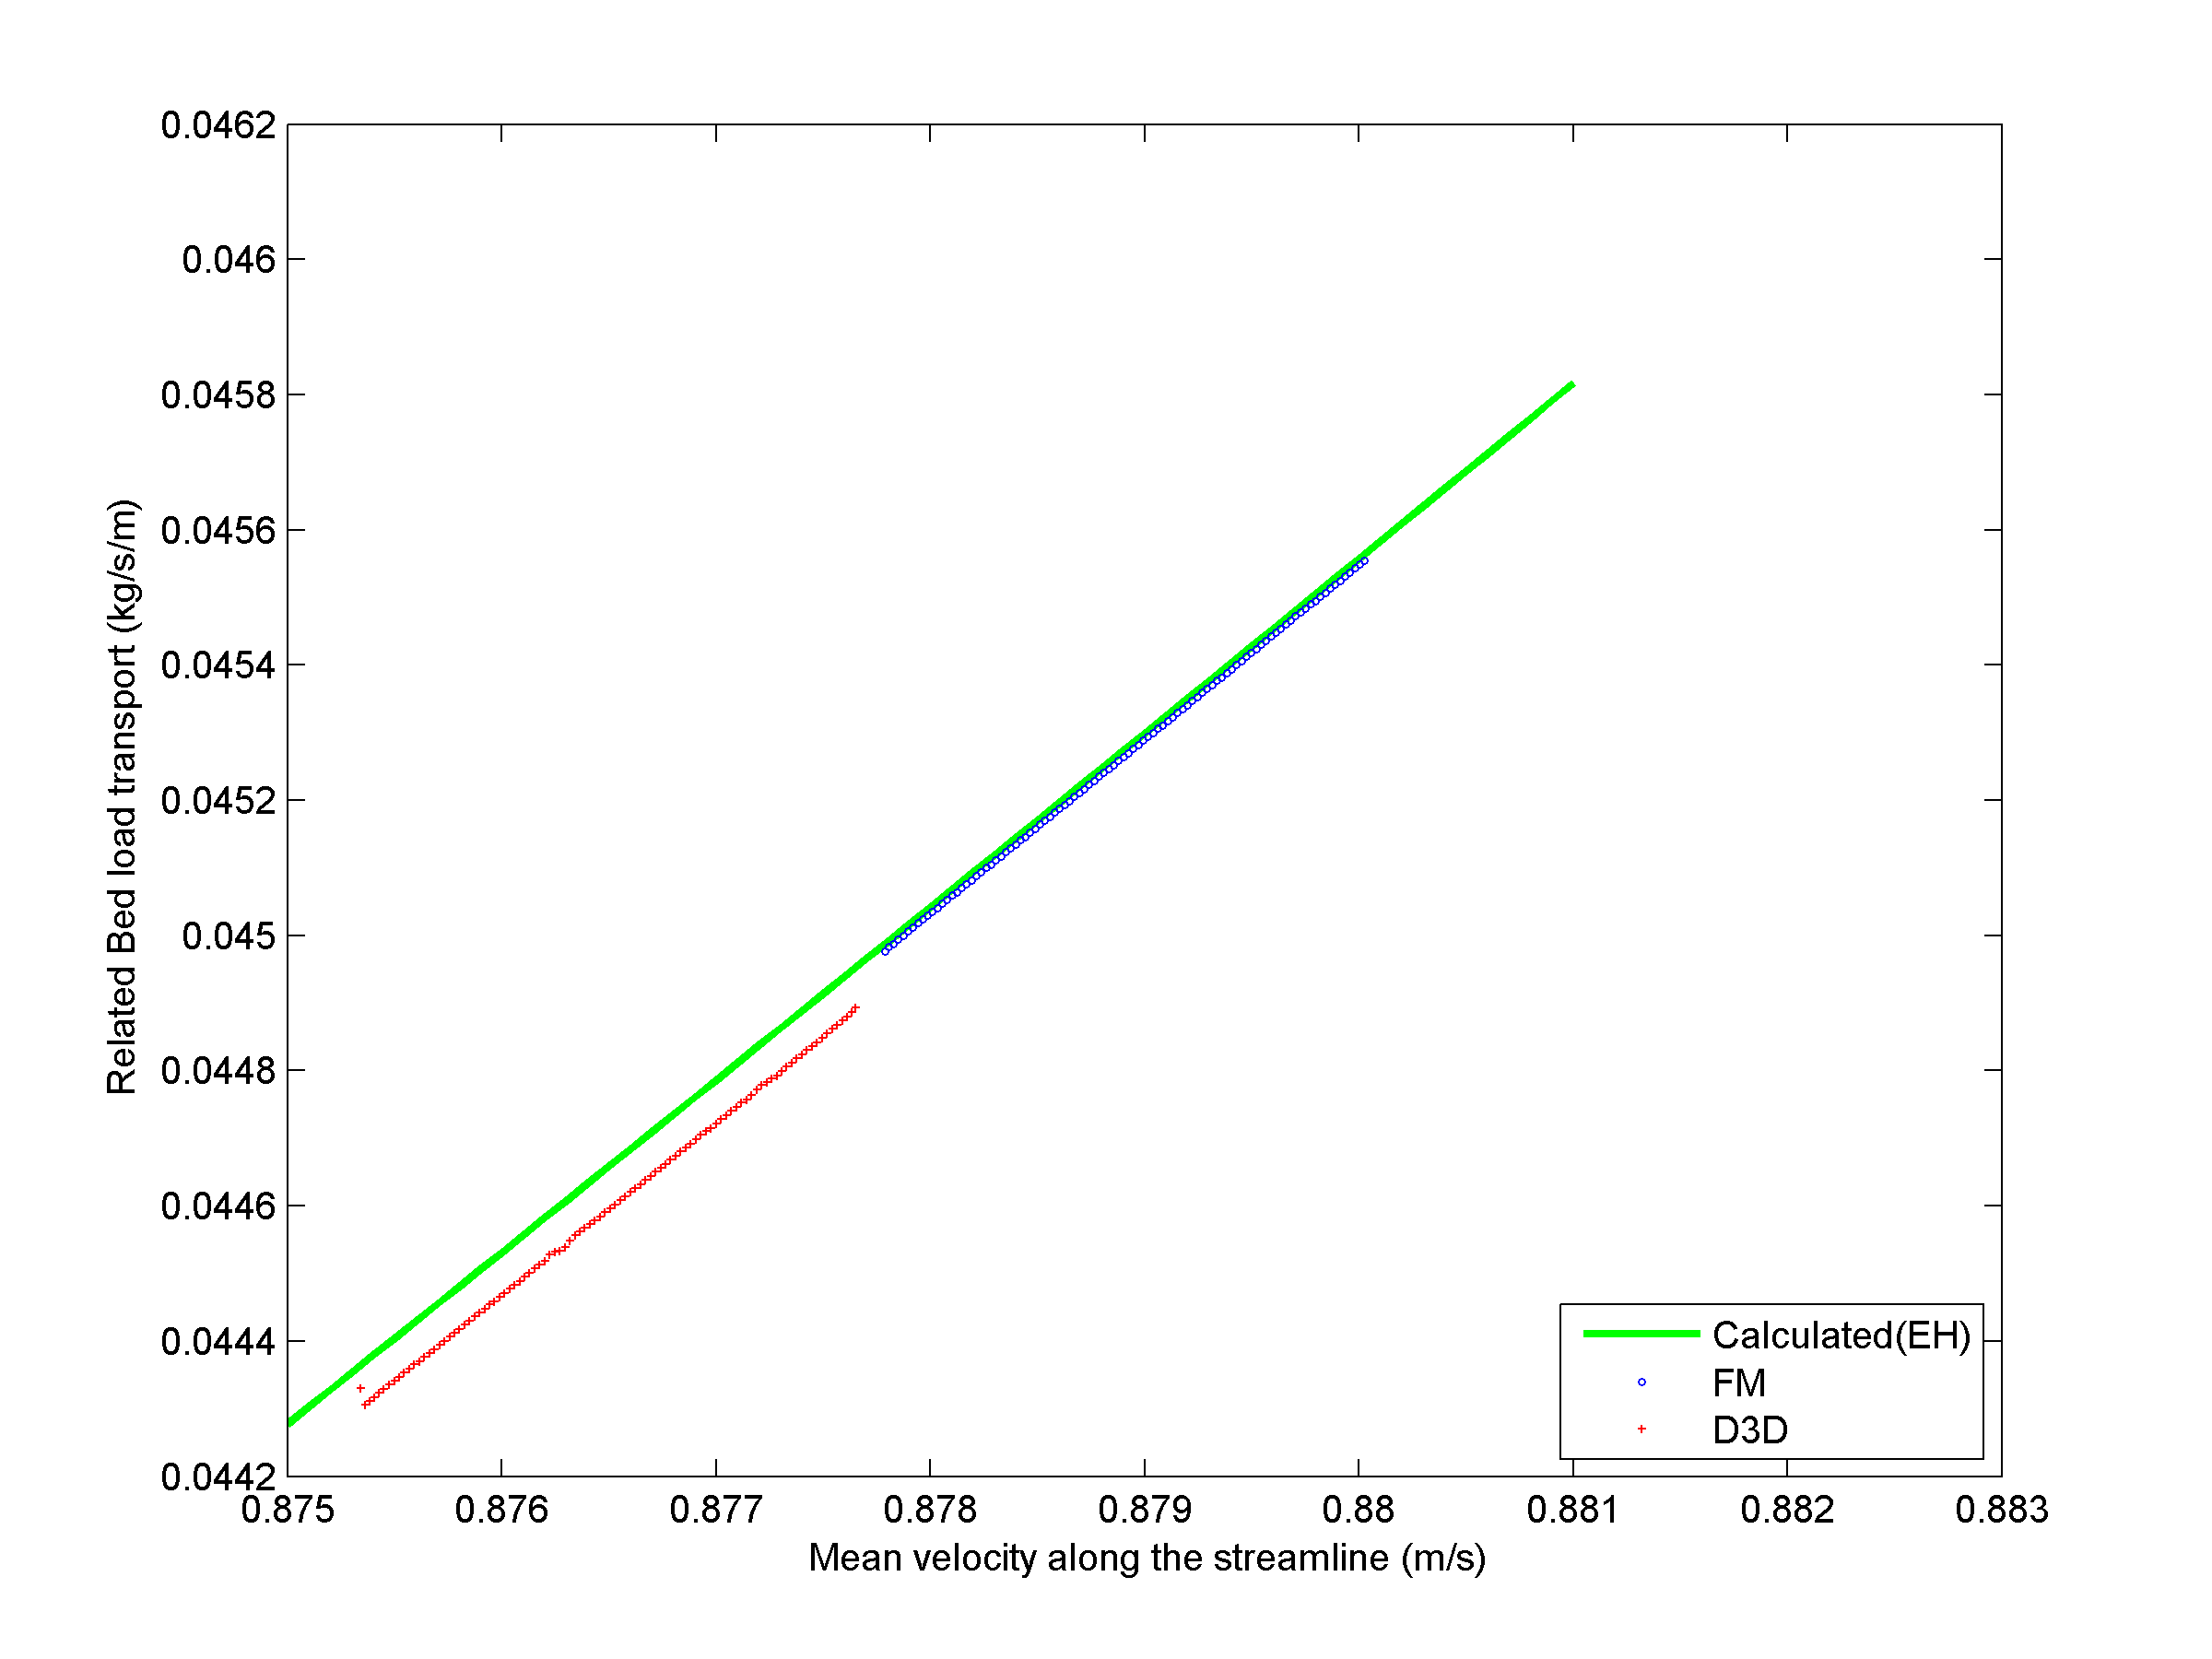
\includegraphics[width=0.7\columnwidth]{velocity_bedloadtransport_plot.png}
    	\end{center}\caption {Comparison of The bedload transport magnitude in the centreline of the straight channel}
    	\label{fig:velocity_bedloadtransport_plot}
    \end{figure} 
    
\paragraph*{Scenarios with morphological changes}
  The scenario of 0.44 transverse slope is used with  activating the morphology and bed composition updates. The simulation is compared with similar simulation using Delft3D software. The results shows that, bed level changes from inclined bed to be more flat due to the erosion and deposition processes executed within both simulations, (Delft3D and FM), as illustrated in the selected cross-section of \Fref{fig:Bedlevel-change}. However, the erosion and deposition processes in Delft3D simulated with more order of magnitude than FM simulation. This would probably occur due to the minor velocity deviation.
  \begin{figure}[h!]
 	\begin{center}	 
 		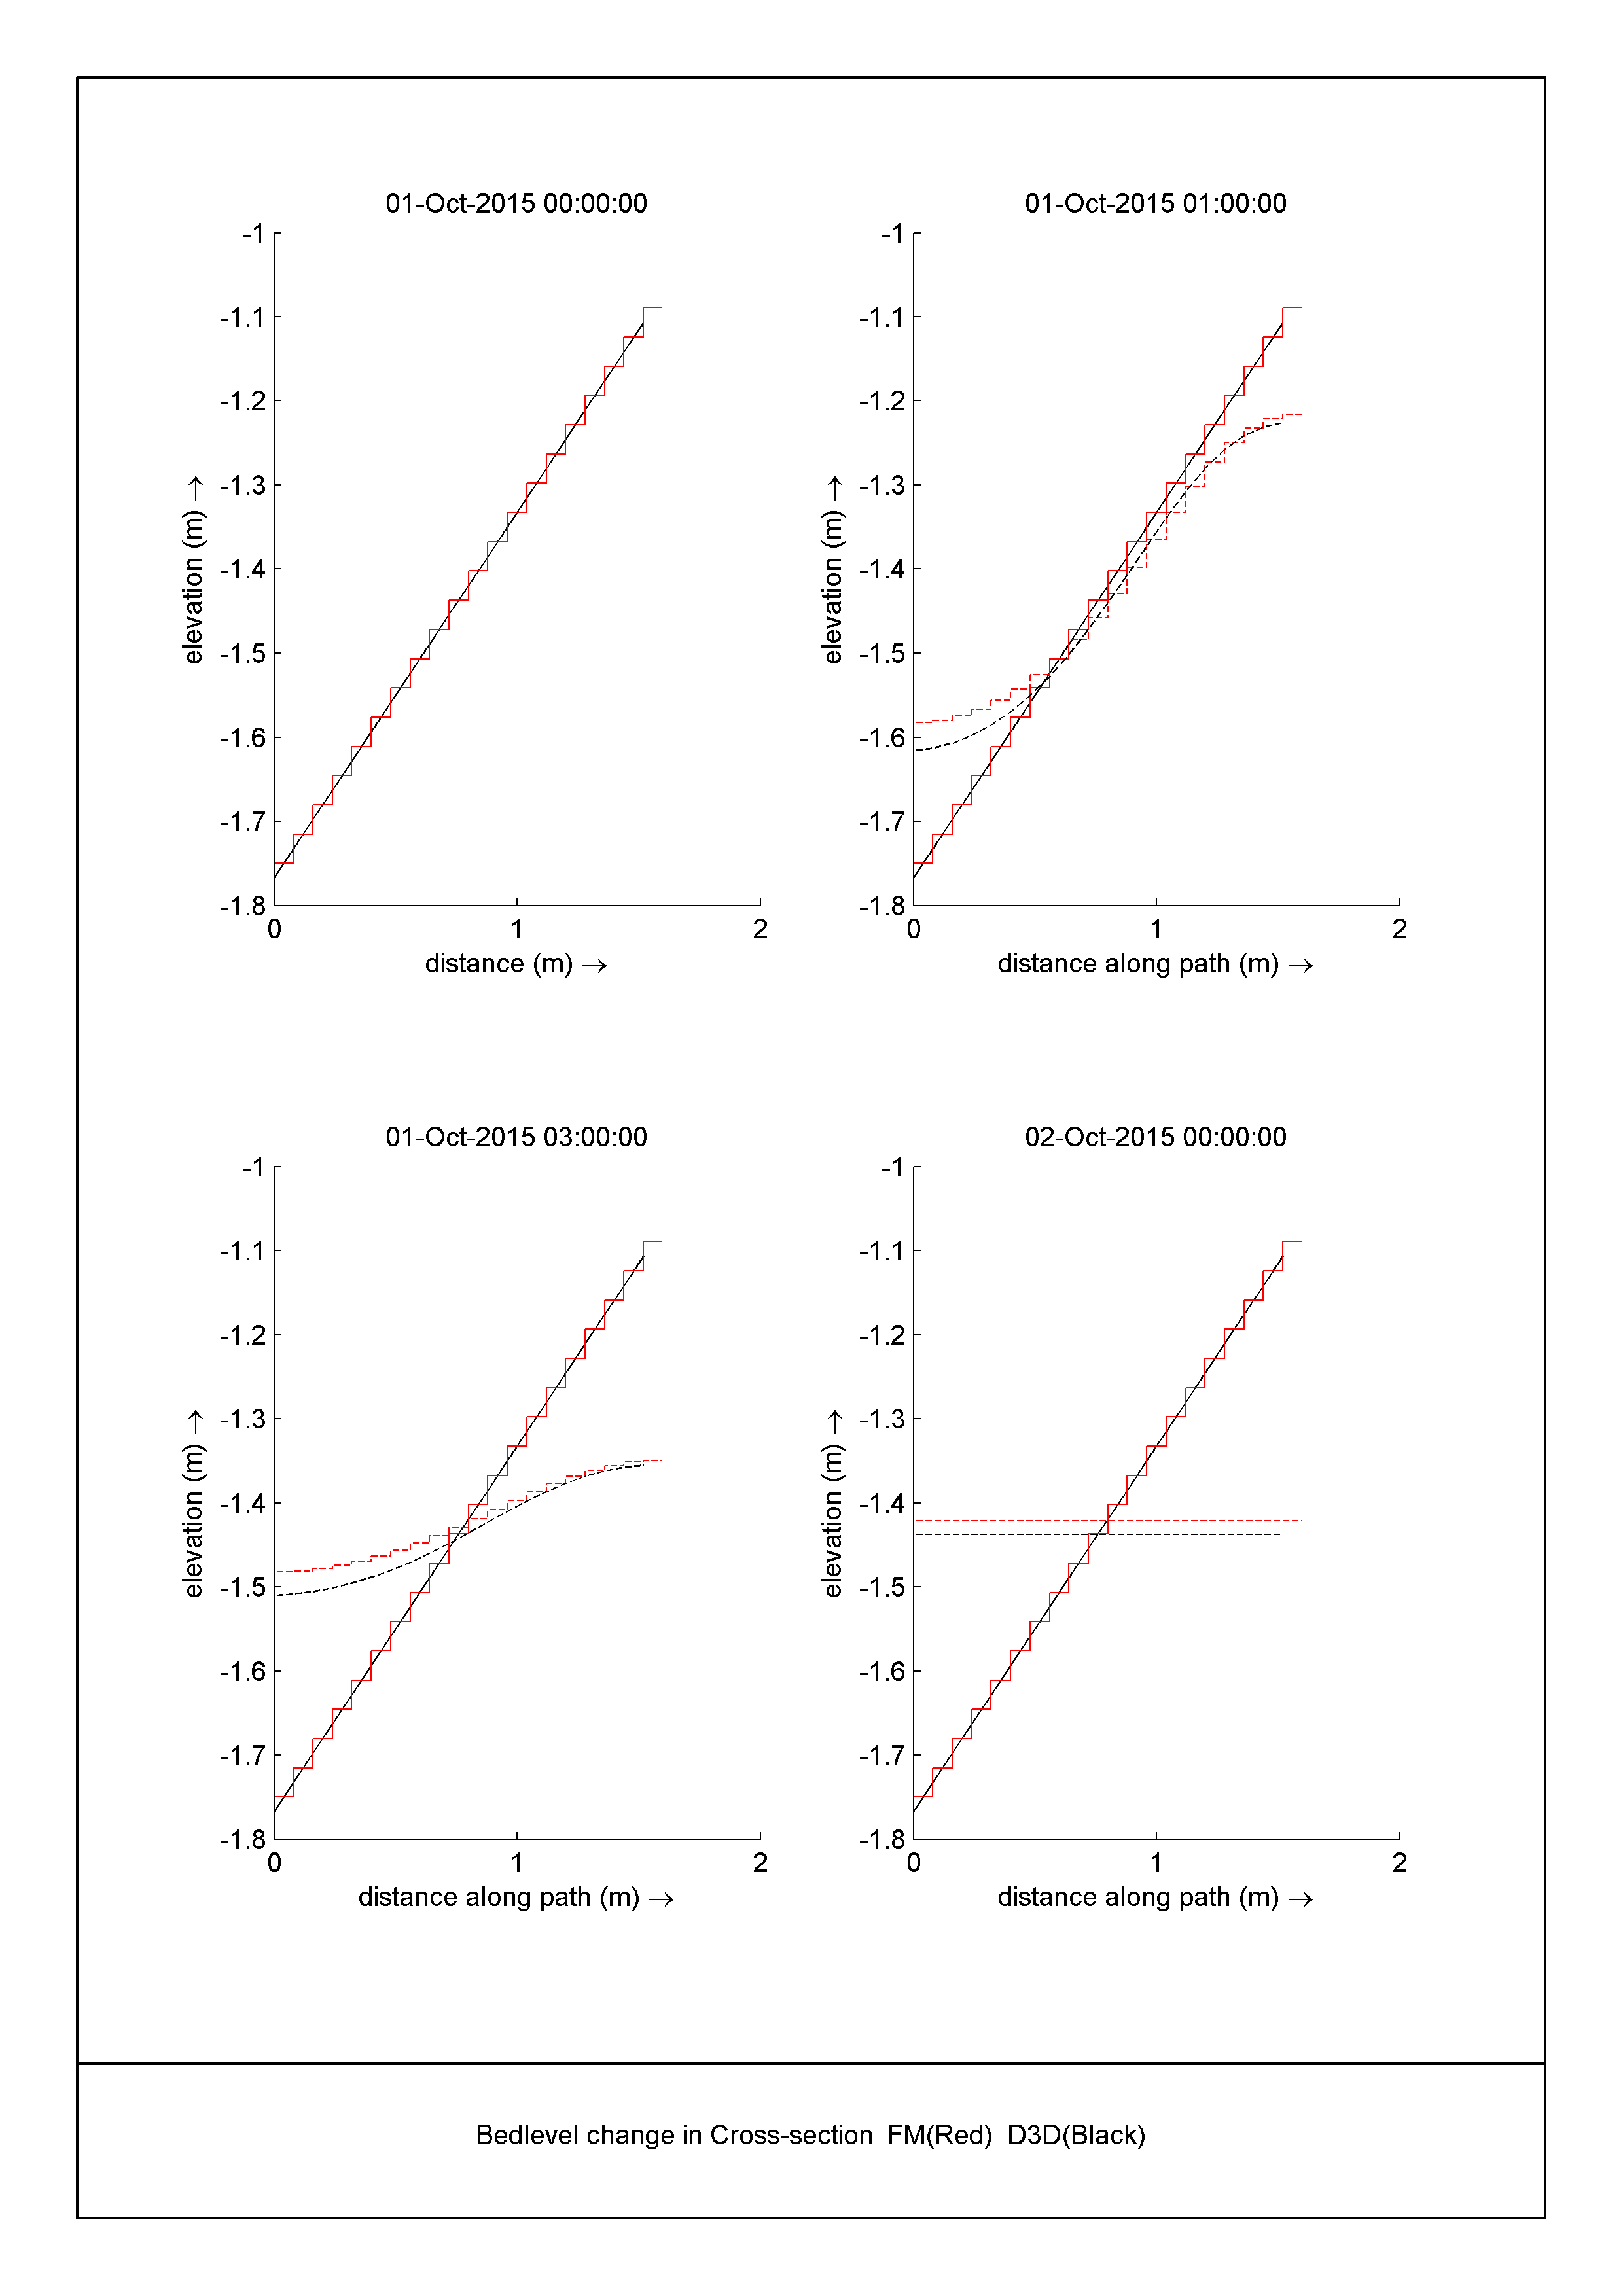
\includegraphics[width=0.7\columnwidth]{Bedlevel-change.png}
 \end{center}\caption {The bedlevel change of a selected cross-section within the channel; Delft3D simulation (Black straight and dotted line) and FM (Red straight and dotted line)}
 	\label{fig:Bedlevel-change}
\end{figure} 
\paragraph*{Results}
The adjusted slope direction of the bedload transport is well represented in flexible mesh with comparison to the Delft3D software.
In addition to that,the difference in bedload transport magnitude between Delft3D simulation and D Flow FM simulations is around 1 to 1.5 $\%$.
This mainly due to the tiny deviation in the velocity magnitude between the two simulations, which is around 0.2 to 0.3 $\%$,since the used transport
 formula is function in the velocity to  power five. Furthermore, the bedlevel change of the FM simulation deviates by 4 to 5$\%$ from Delft3D simulation. 
\paragraph*{Conclusion}
The slope effect module can be used to prescribe bedload transport magnitude and direction. However, in order to get the exact results of Delft3D from D-Flow FM-sed-mor module the above mentioned deviations are to be investigated.
\paragraph*{Version}
This test has been carried out with version dflow-fm-x64-1.1.149.42710.

\if 2 < 1
\fi
\endinput
